\documentclass{ieeeaccess}
\usepackage{cite}
\usepackage{amsmath,amssymb,amsfonts}
\usepackage{algorithmic}
\usepackage{graphicx}
\usepackage{textcomp}

\def\BibTeX{{\rm B\kern-.05em{\sc i\kern-.025em b}\kern-.08em
    T\kern-.1667em\lower.7ex\hbox{E}\kern-.125emX}}
\begin{document}
\history{Date of publication xxxx 00, 0000, date of current version xxxx 00, 0000.}
\doi{10.1109/TQE.2025.DOI}
 
\title{Text Encoding in Quantum Natural Language Processing: A Systematic Survey}

\author{\uppercase{Danilo Cavaliere}\authorrefmark{1}, \uppercase{Giuseppe Fenza}\authorrefmark{1}, \uppercase{Lukasz Gajewski}\authorrefmark{1}, and \uppercase{Vincenzo Loia}\authorrefmark{1}}

\address[1]{Department of Management \& Innovation Systems, Università degli Studi di Salerno, Italy}

\markboth{TEXT ENCODING IN QUANTUM NATURAL LANGUAGE PROCESSING}{TEXT ENCODING IN QUANTUM NATURAL LANGUAGE PROCESSING}

\corresp{Corresponding authors: Danilo Cavaliere and Lukasz Gajewski (e-mails: \{dcavaliere, lgajewski\}@unisa.it).}

\begin{abstract}
Quantum natural language processing (QNLP) applies superposition, entanglement, and interference to the representation and processing of linguistic information. Any QNLP pipeline, whatever methods it uses, must first map discrete or distributed text representations onto qubit registers or parameterized-circuit inputs. This encoding step governs model expressivity, qubit resource requirements, and trainability. However, it is rarely studied as an independent variable, and no standard method brings these evaluation aspects together for analyzing and comparing encodings. This article aims to fill this gap by introducing a classification scheme for text encodings, covering both the encoding used and the experimental evidence 
%reported for it
of its benefits and drawbacks
, that is exploited to 
%and employs it to 
carry out a systematic literature review of text encoding strategies in QNLP. The scope is limited to the encoding step: circuit design, ansatz expressibility, and error correction are covered only where they interact directly with encoding choices. The survey covers 125 studies published between 2021 and 2026, using a protocol based on state-of-the-art guidelines to define the search strategy, eligibility criteria, screening procedure, snowball sampling, and data extraction. The scheme is organized around a unifying taxonomy for analyzing and comparing encodings. Seven encoding families are identified and characterized: four major families, angle, amplitude, syntactic (DisCoCat), and structured feature maps (IQP/ZZ), and three emerging families: data re-uploading, hybrid classical--quantum embedding, and Hamiltonian/observable encoding. Their distribution is analyzed across NLP tasks, simulation and hardware environments, qubit budgets, and reporting practice. Three findings stand out: noiseless circuit simulation dominates the literature, real-hardware execution remains rare, and evaluation is too fragmented across author-chosen datasets, baselines, and metrics for results to be compared between studies. The encoding bottleneck, the dimensionality mismatch between linguistic representations and near-term qubit capacities, is stated explicitly as a basis for resource-efficient QNLP algorithm and hardware design.
\end{abstract}

\begin{keywords}
Encoding bottleneck, parameterized quantum circuits, quantum machine learning, quantum natural language processing, text encoding.
\end{keywords}

\titlepgskip=-15pt

\maketitle

\section{Introduction}
\label{sec:introduction}
\PARstart{E}{very} quantum natural language processing (QNLP) system begins with a mandatory step: converting text into a quantum state. Before a single gate is applied or a single parameter is trained, a token, sentence, or document must be mapped onto qubits. This mapping, the encoding, determines how many qubits are consumed and how deep the resulting circuit must be. It determines whether gradients can be computed efficiently, and whether any genuinely quantum property, such as entanglement, is brought to bear on the linguistic content. It is the most consequential design decision in the pipeline.

Despite this centrality, encoding is rarely the subject of dedicated study: effort concentrates instead on other stages of the pipeline, such as ansatz design \cite{ruskanda_simple_2023,abiwardani_generalized_2025} and the choice of classical optimizer \cite{rajashekharaiah_sentence_2023}, or on carrying QNLP to a new task or domain \cite{abbaszadeh_hybrid_2026,kesiku_unlocking_2026}. Most QNLP papers dispatch it in a paragraph, introduce one strategy without justification, and move on to reporting accuracy numbers. After five years of accelerating publication activity, the result is a fragmented body of work: dozens of encoding families coexist, yet there is no common approach for analyzing and comparing them. Unified taxonomies, systematic comparisons, and a shared understanding of encoding trade-offs are all missing from the literature. Existing QNLP surveys and reviews do not isolate encoding as a variable \cite{chen_survey_2024,pallavi_quantum_2025}. The few explicitly comparative studies contrast model families or ans\"atze rather than encoding schemes \cite{bouakba_comparative_2025,castillo_comparative_2025}. This article fills that gap: it conducts an extensive systematic literature review of the topic and makes text encoding in QNLP the primary subject of study.

\subsection{Scope}
This survey reviews research that (1) applies a genuine quantum circuit (simulated noiseless, simulated noisy, or executed on real hardware) to at least one NLP task, and (2) identifies, at least by name or type, the encoding scheme used to map text or text-derived features onto qubits or circuit parameters. The review follows an SLR protocol defined before the search (Section~\ref{sec:method}) adapted from established guidelines for systematic literature reviews in computer science \cite{keele2007guidelines}.

Papers that use quantum-inspired or quantum-motivated classical algorithms without instantiating an actual parameterized quantum circuit are excluded. Also excluded are survey and review papers, hardware-focused benchmarking studies that treat NLP datasets as a generic payload, and papers whose methodological detail is insufficient to identify the encoding scheme, according to the inclusion and exclusion criteria stated in Section~\ref{sec:criteria}. The final corpus comprises 125 studies.

The scope is limited to the encoding step. Quantum circuit design, ansatz expressibility, and quantum error correction are surveyed only where they interact directly with encoding choices. Classical NLP methods are discussed only as baselines.

\subsection{Research Questions}
\label{subsec:research_questions}

The review is organized around five research questions, each answered from the data extracted across the corpus rather than from the claims of individual studies:

\begin{itemize}
\item[RQ1)] Which text encoding strategies are used in QNLP, and by what principle can they be organized into families? (Section~\ref{sec:taxonomy})

\item[RQ2)] How does the use of each family vary across model families and ans\"atze, and can an encoding be compared independently of the architecture hosting it? (Section~\ref{sec:comparative_analysis})

\item[RQ3)] How has the mix of encodings and architectures changed over the years the corpus spans? (Section~\ref{sec:temporal_evolution})

\item[RQ4)] Does the choice of encoding track the NLP task, and is there a task family whose structure gives a principled reason to prefer one encoding over another? (Section~\ref{sec:task_fit})

\item[RQ5)] How rigorously are encoding claims evaluated, in terms of execution regime, hardware validation, and reproducibility? (Section~\ref{sec:experimental_rigor})
\end{itemize}

\subsection{Key Contributions}
This article makes four contributions to the study of text encoding in QNLP:
\begin{enumerate}
\item[1)] A novel taxonomy of text encoding strategies, organized by the point at which text enters the quantum computation and covering seven encoding families (four major and three emerging) with their specialized variants.
\item[2)] A systematic review of 125 studies that apply or propose quantum text encodings across NLP tasks, conducted under a protocol defined before the search and grounded in established methodological guidelines for systematic literature reviews: the Keele and Charters procedure for systematic reviews in computing \cite{keele2007guidelines}, the PRISMA 2020 statement for reporting the selection process \cite{page2021prisma}, and Wohlin's guidelines for snowball sampling \cite{wohlin2014guidelines}.
\item[3)] A quantitative cross-study characterization of the corpus, spanning encoding-by-model-family, temporal, task-fit, and experimental-rigor analyses.
\item[4)] A characterization of the encoding bottleneck in light of the survey results: the gap between the dimensionality of the text representations studies start from and the qubit budgets they actually use is quantified over the corpus, and each encoding family is read as a choice of which cost absorbs that gap, discarded information, added circuit depth, or a classical burden relocated upstream. This characterization, together with the gaps documented across the review, yields a corpus-derived set of five open challenges and an actionable agenda for future work.
\end{enumerate}

\subsection{Related Work}
\label{subsec:related_work}
Several prior works survey the QNLP literature, but none treats text encoding as the central variable. Varmantchaonala et al.\ \cite{varmantchaonala_quantum_2024} provide the most comprehensive QNLP survey to date, covering quantum algorithms, circuit architectures, and NLP task categories; encoding appears only as an implementation detail. Guarasci et al.\ \cite{guarasci_quantum_2022} offer an early and influential overview of QNLP challenges and opportunities, from theoretical quantum-advantage arguments to hardware experiments, without isolating encoding as a dimension of comparison. Widdows et al.\ \cite{widdows_quantum_2024} examine word embeddings and sequential quantum models with more attention to representation trade-offs than any other general survey, but stop short of a systematic comparison. Bouakba and Belhadef \cite{bouakba_comparative_2025} experimentally compare compositional DisCoCat models against quantum neural networks; their compositional-versus-flat-vector axis overlaps with the taxonomy proposed here, though their scope is limited to two model families. Huzzat et al.\ \cite{huzzat_primer_2026} is the most encoding-aware prior work: it addresses the mismatch between text-representation dimensionality and the qubit capacity of NISQ classifiers, and treats classical compression as a prerequisite for stable training. It remains, however, a conceptual primer for a single model class rather than a systematic review.

Beyond QNLP itself, the quantum engineering literature has an established tradition of comprehensive subfield surveys, covering, for instance, quantum circuit compilation for NISQ devices \cite{kusyk2021survey}, quantum computing for finance \cite{egger2020quantum}, and entanglement routing in quantum networks \cite{abane2025entanglement}, the last of which likewise organizes its field through an explicit taxonomy of approaches. None of these addresses text encoding in QNLP, which is the gap the present survey fills within that tradition.

This survey complements these works by treating encoding as the primary unit of analysis, yielding the first quantitative cross-study characterization of how text is encoded in QNLP and at what resource cost.

\subsection{Structure}
The rest of the article is organized as follows. Section~\ref{sec:background} provides the background on quantum computing, compositional distributional semantics, and the role of encoding in QNLP. Section~\ref{sec:method} describes the systematic review protocol (search strategy, eligibility criteria, screening, and snowball sampling) and the data extraction and classification scheme used throughout the analysis. Sections~\ref{sec:taxonomy}--\ref{sec:experimental_rigor} then answer RQ1--RQ5 in turn. Section~\ref{sec:trends_challenges} synthesizes the trends, states the encoding bottleneck explicitly, and enumerates the open challenges and the future-work agenda. Section~\ref{sec:conclusion} concludes.

\section{Background}
\label{sec:background}

\subsection{Quantum Computing Primitives}

A quantum bit (qubit) occupies a superposition of the basis states $|0\rangle$ and $|1\rangle$:
\begin{equation}
|\psi\rangle = \alpha|0\rangle + \beta|1\rangle, \quad |\alpha|^2 + |\beta|^2 = 1,
\end{equation}
where $\alpha, \beta \in \mathbb{C}$ are probability amplitudes. A register of $n$ qubits occupies a $2^n$-dimensional Hilbert space $\mathcal{H} = \mathbb{C}^{2^n}$; its state is a unit vector in that space. This exponential dimension is the property every amplitude-style encoding exploits. Entanglement introduces correlations with no classical counterpart, and measurement collapses the state to a classical bitstring, destroying superposition. Whether superposition, entanglement, or interference confers a practical benefit on NLP tasks remains the central open question of the field, and Section~\ref{sec:experimental_rigor} examines how far the surveyed evidence can speak to it.

\subsection{Parameterized Quantum Circuits}

The dominant computational model in near-term quantum machine learning is the parameterized quantum circuit (PQC), also called a variational quantum circuit \cite{cerezo2021variational}. A PQC applies a sequence of unitary gates to an initial state $|\psi_0\rangle$:
\begin{equation}
U(\boldsymbol{\theta}) = U_L(\boldsymbol{\theta}_L) \cdots U_1(\boldsymbol{\theta}_1),
\end{equation}
where $\boldsymbol{\theta} \in \mathbb{R}^p$ are trainable parameters. Model outputs are expectation values $\langle O \rangle = \langle \psi_0 | U^\dagger(\boldsymbol{\theta})\, O\, U(\boldsymbol{\theta}) | \psi_0 \rangle$, and gradients follow analytically from the parameter-shift rule \cite{mitarai2018quantum, schuld2019evaluating}. PQCs underlie six of the seven encoding families surveyed here; the exception is grammatical encoding, which derives circuit structure from sentence syntax rather than from a fixed ansatz.

PQCs operate under the constraints of noisy intermediate-scale quantum (NISQ) hardware \cite{preskill2018quantum}: shallow circuits, limited qubit counts, and significant gate error rates. These constraints bear directly on the encoding step. Every qubit or gate layer spent loading a text representation is a resource unavailable to the learning task.

\subsection{Text Encoding}

Text encoding is the procedure that maps a text input $x$ (a token, sentence, or document) to a quantum state $|\phi(x)\rangle \in \mathcal{H}$ or to a parameter vector $\boldsymbol{\theta}(x)$ that initializes a PQC. It is the mandatory interface between classical language data and the quantum circuit. The input $x$ may be a raw token sequence, a classical embedding vector from a pre-trained model, or a parse tree carrying grammatical structure. Which representation is used, and how it is loaded onto qubits, defines the encoding family.

\subsection{Compositional Distributional Semantics and DisCoCat}

One of the two main traditions in QNLP originates in categorical linguistics. Coecke, Sadrzadeh, and Clark \cite{coecke2010mathematical} showed that the compact closed categorical structure of pregroup grammars also governs quantum processes in Hilbert space. In a pregroup grammar, each word carries a grammatical type, and a sentence is parsed by reducing compound types through tensor contractions. These reductions obey the same diagrammatic calculus as quantum processes, so a parse tree translates directly into a quantum circuit: words become parameterized quantum states, and grammatical reductions become cups in a string diagram.

This is the DisCoCat (Distributional Compositional Categorical) model, operationalized as an end-to-end pipeline by \cite{lorenz_qnlp_2023} and executed on near-term hardware in \cite{meichanetzidis_quantum_2021, meichanetzidis_grammar-aware_2023} via the \textsc{lambeq} toolkit. The circuit structure is not fixed in advance: the parse tree determines it, so syntactically distinct sentences produce structurally distinct circuits. This property sets the grammatical encoding family apart from all other families, which treat the sentence as a flat feature vector.

\subsection{Quantum Machine Learning for Text}

The second tradition approaches NLP as a classification problem. It applies quantum feature maps \cite{schuld2019quantum} and variational circuits \cite{cerezo2021variational} to text-derived feature vectors: classical embeddings (word2vec, GloVe, or transformer outputs) are compressed to the available qubit count, loaded into a PQC via rotation gates or amplitude encoding, and trained end-to-end on labeled examples. Because this approach assumes nothing about grammatical structure, it applies to arbitrary text without a parser and scales more easily to realistic dataset sizes. Its logical endpoint is the hybrid quantum--classical architecture, in which a large classical language model handles high-dimensional representation and a small quantum circuit acts as a downstream head; such architectures have grown in prevalence since 2023.

The two traditions differ in how they encode text and in what they claim the quantum component contributes. Compositional models argue for structural alignment between grammar and quantum computation; QML models argue for expressivity or kernel separability.

\begin{figure*}[t]
\centering
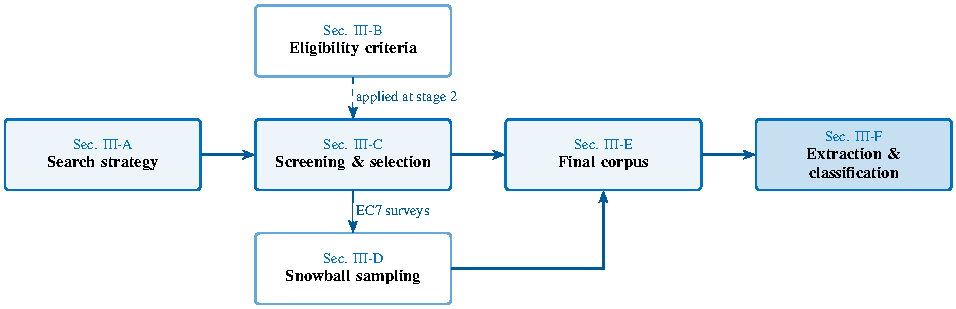
\includegraphics[width=\textwidth]{figures/fig_method.pdf}% built from fig_method.tex
\caption{Overview of the review methodology. Each block corresponds to the subsection that details it (full selection flow in Fig.~\ref{fig:prisma}).}
\label{fig:method}
\end{figure*}

\section{Review Methodology}
\label{sec:method}

This systematic literature review followed the guidelines for systematic
literature reviews in software engineering established by Keele and
Charters~\cite{keele2007guidelines}. According to these principles, the protocol for paper collection and analysis was defined by fixing
%before the search was executed. It fixed 
the search strategy, eligibility criteria, screening
procedure, snowball sampling, and data extraction process. All these stages are part of the collection pipeline that is summarized in Fig.~\ref{fig:method}. Each stage is detailed in the rest of this section.

\subsection{Search Strategy}
\label{subsec:search}

Two complementary search queries were executed on the primary bibliographic databases (e.g., Scopus, IEEE Xplore), to cover both the quantum machine learning and the
compositional QNLP literature. The first query targeted the intersection of
quantum computing or machine learning with NLP and encoding-related terms. The
second targeted QNLP-specific terminology: the DisCoCat and DisCoCirc
frameworks, established pipelines that implement them such as the lambeq
toolkit, and categorical linguistic concepts. The searches were restricted to
English-language journal articles and conference papers published between 2021
and 2026 (ends included), excluding editorials, book chapters, and erratum
notices. They returned 269 results from Scopus and 217 from IEEE Xplore, a
combined total of 486 records. Removing 110 duplicates left 376 unique records.

\subsection{Eligibility Criteria}
\label{sec:criteria}

A study was selected if and only if it met all six inclusion criteria below.
\begin{itemize}
\item \textit{IC1: NLP task grounding.} The study applies or evaluates the
  proposed method on at least one natural language processing task, such as
  classification, similarity, sequence labeling, question answering, or
  generation.
\item \textit{IC2: Genuine quantum computation.} The study implements and
  evaluates the method in at least a noiseless quantum circuit simulation
  (exact statevector simulation or equivalent) or on real quantum hardware;
  merely quantum-inspired classical algorithms, such as tensor-network models
  or classical approximations of quantum kernels, do not satisfy this
  criterion.
\item \textit{IC3: Encoding scheme identified.} The study names or identifies
  at least the type of encoding used to map text or text-derived features onto
  qubits, quantum states, or circuit parameters; a named or typed mention is
  sufficient, and circuit diagrams or full mathematical derivations are not
  required.
\item \textit{IC4: Peer-reviewed or preprint venue.} The study appeared in a
  peer-reviewed journal, conference, or workshop, or as a preprint with
  sufficient methodological detail to assess IC1--IC3.
\item \textit{IC5: Language and access.} The study is available in full text,
  in English, and accessible for review.
\item \textit{IC6: Time window.} The study was published between 2021 and 2026
  inclusive.
\end{itemize}
Even if a study satisfied all six inclusion criteria, it was excluded if any of
the following applied:
\begin{itemize}
\item \textit{EC1: No NLP application.} The study applies quantum machine
  learning exclusively to non-text domains and offers no transferable
  text-encoding discussion.
\item \textit{EC2: Classical-only encoding.} The study uses encoding purely in
  the classical sense (tokenization, positional encoding, one-hot) with no
  quantum circuit involved.
\item \textit{EC3: Insufficient detail.} The study is an abstract, extended
  abstract, or short paper that names an encoding but provides no formal
  description or reproducible detail.
\item \textit{EC4: Duplicate or superseded.} The study is a conference version
  superseded by an extended journal version; only the more complete version
  was retained.
\item \textit{EC5: Pure hardware focus.} The study addresses hardware
  benchmarking alone and uses an NLP dataset only as a generic payload, with no
  discussion of linguistic encoding properties.
\item \textit{EC6: Quantum-inspired, classical surrogate, or unverifiable
  simulation.} The study uses quantum-derived mathematical formalism without
  instantiating an actual parameterized quantum circuit, reports only classical
  surrogates of quantum behavior, or claims quantum simulation without evidence
  of framework or circuit use.
\item \textit{EC7: Survey or review paper.} The study is primarily a survey or
  review of existing work rather than an original research contribution; such
  papers were retained as reference material and are discussed in
  Section~\ref{subsec:related_work}.
\end{itemize}

\subsection{Screening and Selection}
\label{subsec:screening}

Screening proceeded in two stages. In the first stage, all 376 records were
assessed on title and abstract alone for broad topical relevance to quantum
computing applied to text. No IC/EC criteria were applied at this stage; its
only purpose was to remove records clearly outside the scope of the review.
This eliminated 234 records and left 142 reports sought for retrieval, of which
6 could not be retrieved, leaving 136 reports assessed for eligibility.

In the second stage, the full text of each of the 136 reports was assessed
against the complete set of inclusion and exclusion criteria of
Section~\ref{sec:criteria}. This yielded 95 papers for the corpus. The
remaining 41 retrieved reports were excluded or retained as surveys, mainly
under IC2 (no genuine quantum circuit; $n = 15$), IC3 (encoding scheme not
identified; $n = 6$), EC6 (quantum-inspired, classical surrogate, or
unverifiable simulation; $n = 3$), and EC7 (survey or review; $n = 11$); six
records were excluded under other criteria.

\subsection{Snowball Sampling}
\label{subsec:snowball}

To reduce the risk of missing relevant work not indexed by the two databases,
two rounds of backward and forward snowball sampling~\cite{wohlin2014guidelines} were
applied to the surveys excluded under EC7. Surveys were chosen as the seed set,
rather than the included studies, for two reasons. First, Wohlin's guidelines
ask for a start set that is small, diverse, and well connected to the target
population; in a field as young as QNLP, the reference list of a survey is by
construction a curated, near-exhaustive sample of the literature in the field
up to its search date, so each survey seed contributes far more unique
candidates than an individual study, whose citations concentrate on the same
few foundational works. Second, forward snowballing from surveys exploits a
stable citation practice: new studies routinely cite the reviews of the field,
so the papers citing a survey are enriched for precisely the recent work that
database indexing lags behind. The cost of this choice is that a study neither cited by nor citing any
survey of the field remains invisible to the procedure. Reference lists and citing papers
yielded 1222 unique candidate records. Title-and-abstract screening for broad
topical relevance reduced this set to 242 reports sought for retrieval, of
which 37 could not be retrieved, leaving 205 reports assessed for eligibility.
Full-text assessment against the complete IC/EC protocol then added 30 papers
to the corpus. The remaining 175 retrieved reports were excluded or retained as
surveys. The main grounds were IC1 (no NLP task; $n = 74$), IC2 (no genuine
quantum circuit; $n = 52$), IC6 (outside the time window; $n = 20$), IC3
(encoding scheme not identified; $n = 4$), and EC7 (survey or review;
$n = 22$); three records were excluded under other criteria.

\subsection{Final Corpus}
\label{subsec:corpus}

\begin{figure*}[t]
\centering
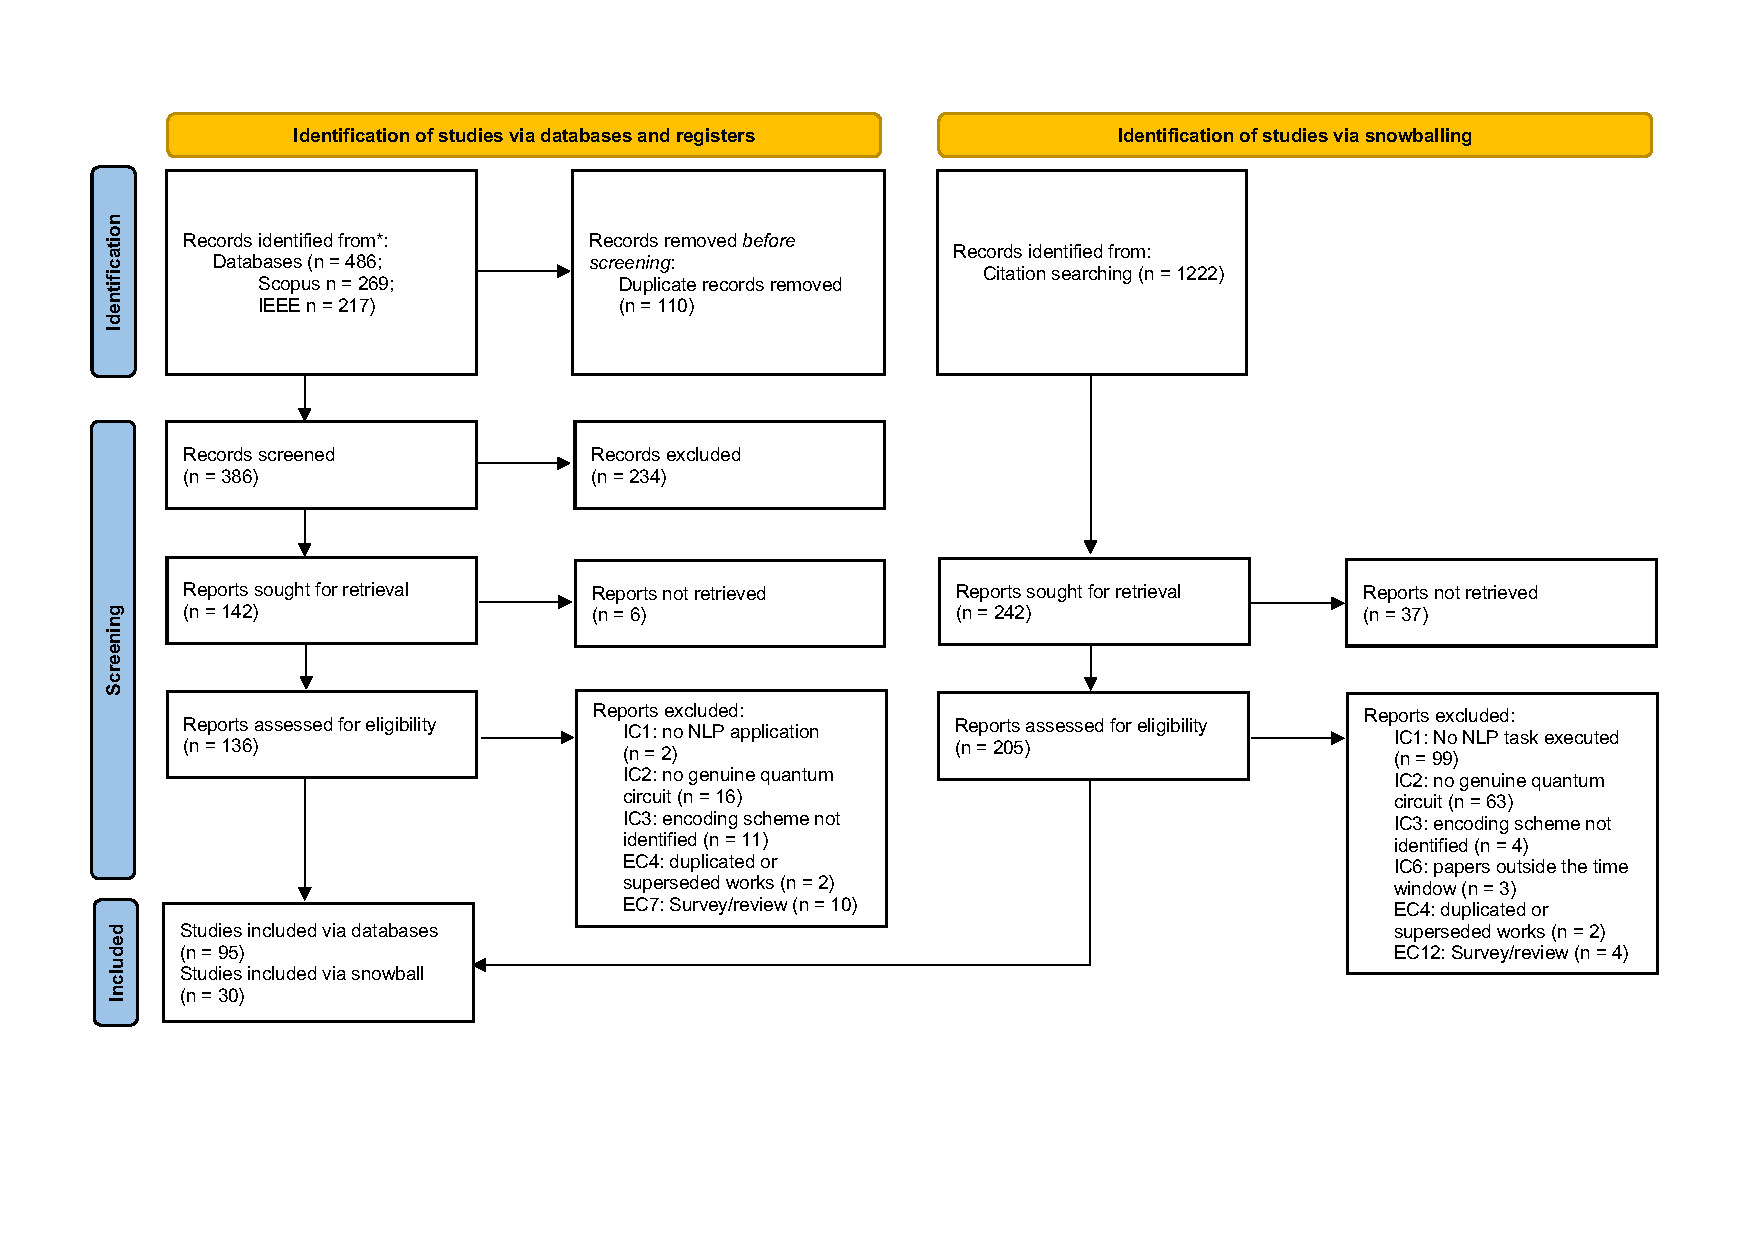
\includegraphics[width=\textwidth]{figures/PRISMA_Chart.pdf}
\caption{PRISMA flow diagram. Final corpus: $n = 125$ (95 from database search,
30 from snowball sampling).}
\label{fig:prisma}
\end{figure*}

The final corpus comprises 125 papers, 95 from the database search and 30 from
snowball sampling; Fig.~\ref{fig:prisma} summarizes the selection process as a
PRISMA 2020 flow diagram~\cite{page2021prisma}.

\subsection{Data Extraction and Classification}
\label{subsec:analysis_framework}

Each study in the corpus was classified along a fixed set of dimensions, so
that every classification, cross-tabulation, and trend reported in
Sections~\ref{sec:taxonomy}--\ref{sec:trends_challenges} follows directly from the extraction sheet rather than from an
ad hoc reading of the corpus. The two primary dimensions are the encoding
family, defined by the point at which text or text-derived features enter the
quantum computation (Section~\ref{sec:taxonomy}), and the model family, defined by the
architecture that consumes the encoded state. Secondary dimensions capture the
resources and evidence attached to that choice: qubit count and whether qubit
scaling was tested, execution regime, presence of a classical baseline, and
whether scalability was discussed. Each dimension is operationalized as one or
more columns of the structured extraction sheet compiled during data
extraction.

Assignment follows explicit decision rules. A study is classified by its
dominant encoding interface: the one that carries the text representation into
the circuit whose output is evaluated. Auxiliary encodings used only in
ablations or baselines do not change the class; a study whose main pipeline is
amplitude-encoded but that reports an angle-encoded ablation is classified as
amplitude. Where a pipeline stacks a classical encoder in front of a quantum
layer, the study is classified as \texttt{hybrid\_embed} only when the
classical stage is co-trained or purpose-built as part of the contribution; a
frozen pretrained embedding feeding a standard rotation layer remains
\texttt{angle}. The \texttt{hybrid\_nn} model family covers any architecture in
which a classical deep network (transformer, recurrent, or convolutional, not
limited to LLM-based extractors) performs the main representational work and
the quantum circuit is a submodule. A bare variational classifier over
precomputed features is \texttt{vqc}, even when those features come from a deep
model. Compositional (DisCoCat-style) studies are identified by circuit
topology derived from a grammatical parse, regardless of toolkit. These
disambiguation rules were fixed during protocol definition and applied
uniformly during extraction.

All figures below are reported over the full corpus of 125 studies.

The corpus is small enough that many of the cross-tabulations below have cells
in the low single digits, and every count is a complete enumeration of the
corpus rather than an estimate from a sample of it. All distributions are
therefore reported descriptively, as counts and shares of a known population.
Where the article asserts that two dimensions are coupled rather than simply
describing one, the claim rests on the size of the imbalance in the
cross-tabulation together with a stated mechanism, and both are given.
Percentages computed on denominators below ten are reported with their
denominators and are not read as evidence of a difference.

\section{Taxonomy of Text Encoding Strategies}
\label{sec:taxonomy}

%STEP 1 remind the RQ
This section answers RQ1 asking which text encoding strategies are used in QNLP, and by what principle they can be organized into families. The encoding problem in QNLP is not a single operation. Depending on the study, text can enter the quantum computation as rotation parameters, as amplitudes of a prepared state, as a grammar-derived circuit, as a structured feature map, or through a more specialized interface such as repeated data injection, a hybrid neural representation, or an observable. These mechanisms are often discussed under the term ``encoding,'' although they make different assumptions about where linguistic information is represented and which quantum resource is being used.

%STEP 2: Explain how the RQ is tackled
To answer RQ1, this section shows how the above-mentioned mechanisms are organized into the proposed taxonomy as shown in Table~\ref{tab:encoding_taxonomy}, and applying the classification rules presented in Section~\ref{subsec:analysis_framework}.
%STEP 3: discuss the problem
The taxonomy comprises seven encoding families. 
Four are major: 
\begin{itemize}
    \item angle encoding (51 papers),
    \item amplitude encoding (28 papers),
    \item syntactic/DisCoCat encoding (29 papers),
    \item structured feature-map encoding (9 papers).
\end{itemize}
%angle encoding ($n=51$), amplitude encoding ($n=28$), syntactic/DisCoCat encoding ($n=29$), and structured feature-map encoding ($n=9$). 
%Three are emerging families that together account for the remaining eight studies: 
Three are emerging:
\begin{itemize}
    \item data re-uploading (4 papers), 
    \item  hybrid classical--quantum embedding (3 papers),
    \item  and Hamiltonian/observable encoding (1 paper).
\end{itemize}
%data re-uploading ($n=4$), hybrid classical--quantum embedding ($n=3$), and Hamiltonian/observable encoding ($n=1$). 
By using the taxonomy for each approach, one may first identify whether the text representation is loaded as a flat vector, imposed through linguistic structure, or used to define a kernel geometry. The next design question is whether the encoding is intended to minimize qubit count, preserve linguistic composition, define a kernel geometry, or improve trainable circuit expressivity. Not all combinations are equally practical on near-term devices. The main tradeoff is between width, depth, state-preparation cost, and the amount of linguistic structure preserved by the quantum circuit \cite{preskill2018quantum,cerezo2021variational,ruskanda_evaluating_2025}. This approach is used in the rest of the section to analyze each method per encoding family to answer RQ1. 

\begin{table*}[t]
\caption{Taxonomy of text encoding strategies in the final corpus: four major families and three emerging families.}
\label{tab:encoding_taxonomy}
\centering
\scriptsize
\begin{tabular}{@{}p{0.18\textwidth} p{0.09\textwidth} p{0.45\textwidth} p{0.20\textwidth}@{}}
\hline
\textbf{Encoding family} & \textbf{Corpus count} & \textbf{Core mechanism} & \textbf{Typical model families} \\
\hline
\multicolumn{4}{@{}l}{\emph{Major families}} \\
Angle encoding & 51 & Text features are mapped to single-qubit rotation parameters, typically through $R_x$, $R_y$, or $R_z$ gates. & VQC, hybrid neural, recurrent neural, quantum transformer \\
Amplitude encoding & 28 & A normalized feature vector is loaded into the amplitudes of an $n$-qubit state in a $2^n$-dimensional Hilbert space. & VQC, quantum kernel, quantum transformer, hybrid neural \\
Syntactic/DisCoCat encoding & 29 & Sentence grammar determines a string diagram or circuit; word meanings are attached to grammatical types and composed by reductions. & Compositional QNLP \\
Structured feature maps & 9 & Classical text features parameterize structured circuits such as IQP, ZZFeatureMap, ZFeatureMap, PauliFeatureMap, or Pauli-Y variants. & Quantum kernel, VQC, hybrid neural, quantum transformer \\
\multicolumn{4}{@{}l}{\emph{Emerging families}} \\
Data re-uploading & 4 & Input features are injected repeatedly across circuit layers, alternating data-dependent rotations with trainable transformations. & VQC, recurrent neural \\
Hybrid embedding & 3 & A classical encoder first produces a compact text representation that is then passed to a quantum layer. & Hybrid neural, VQC \\
Hamiltonian/observable encoding & 1 & Text-derived information is represented through Pauli-string Hamiltonians or observables rather than only through prepared quantum states. & VQC \\
\hline
\end{tabular}
\end{table*}

\subsection{Angle Encoding}
\label{subsec:angle_encoding}

%STEP 1: introduce the encoding
Angle encoding is the dominant category in the corpus. In this scheme, a classical vector $\mathbf{x} = (x_1,\ldots,x_d)$ is mapped to rotation parameters,
\begin{equation}
|\phi(\mathbf{x})\rangle =
\prod_{j=1}^{d'} R_{\alpha_j}(s_j(\mathbf{x})) |0\rangle^{\otimes n},
\end{equation}
where $R_{\alpha_j}$ is a rotation around the $x$, $y$, or $z$ axis and $s_j(\cdot)$ denotes scaling, projection, or feature selection. The input is rarely raw text. It is usually a TF-IDF vector, a word or sentence embedding, a transformer representation, or a compact feature vector produced by a preceding classical model.

%STEP 2: discuss its details (use itemize, pointed lists, figures, etc. to get it short)
The prevalence of angle encoding follows from its implementation simplicity. Rotations fit naturally into parameterized quantum circuits and support the standard gradient-based training workflow of variational algorithms, and they avoid arbitrary-state preparation, which makes them convenient for small simulated or hardware-oriented experiments \cite{mitarai2018quantum,schuld2019evaluating}. What makes the family a single encoding category is this shared rotation mechanism; within it, the corpus studies differ along two encoding-level axes: the rotation construction itself and the classical source that supplies the angles. 

\begin{itemize}
    \item \textbf{First Axis: Rotation Construction.} The most common pattern assigns one feature to one single-axis rotation, typically an $R_Y$ rotation as in the default angle-embedding routine \cite{ruskanda_evaluating_2025,kesiku_quantum_2025,diaz-ortiz_strongly_2024}, though $R_X$ is also used \cite{day_qnet_2023,zhou_new_2022,tiwari_quantum_2024} and some studies apply combined $R_Y$ and $R_Z$ rotations per qubit \cite{stein_applying_2023}. A denser variant stores more than one feature on each qubit through successive rotations about different axes, trading a shorter register for greater loading depth \cite{kesiku_unlocking_2026}.
    \item \textbf{Second Axis: Classical source of the angles.} This is the aspect on which the studies vary the most, because the rotation parameters are numbers rather than text and so the content of the encoding is fixed by the front-end that produces them. Some studies load sparse lexical statistics such as TF-IDF, bag-of-words, or $n$-gram vectors \cite{boopalamani_quantum-enhanced_2025,payares_quantum_2023,kabir_qtopic_2026}; others load static word embeddings \cite{di_sipio_dawn_2022,diaz-ortiz_strongly_2024,ohno_quantum_2025}; and a large, growing group compresses contextual transformer embeddings, for instance reducing a 768-dimensional BERT or DistilBERT vector to a handful of features before rotation \cite{ahmad_hybrid_2023,kumar_hybrid_2026,suleiman_hdqe_2026,yu_application_2024}. A further group derives the angles from deeper classical feature extractors or from handcrafted linguistic features \cite{rezaei_hybrid_2026,mukesh_qvila_2024,mompelat_compact_2026}. In each case a dimensionality-reduction step, whether PCA, a linear projection, or an autoencoder, sits between the text representation and the rotations and is effectively part of the encoding, since it determines what survives into the quantum circuit.
\end{itemize}

%STEP 3: Benefits and drawbacks
The limitation is inherent in this design. Encoding cost grows with the number of retained features, so a model must spend more rotations, more qubits, or more layers as it keeps more of the input. Angle encoding therefore pushes the hard part of the problem onto classical dimensionality reduction, which makes it practical for NISQ-scale prototypes but also means the quantum circuit often operates on a heavily compressed view of the linguistic input.


\subsection{Amplitude Encoding}
\label{subsec:amplitude_encoding}

%STEP 1: introduce the encoding
Amplitude encoding maps a normalized vector $\mathbf{x} \in \mathbb{R}^{2^n}$ or $\mathbb{C}^{2^n}$ to a quantum state,
\begin{equation}
|\phi(\mathbf{x})\rangle = \sum_{i=0}^{2^n-1} x_i |i\rangle,
\quad \sum_i |x_i|^2 = 1.
\end{equation}
For NLP, the appeal is immediate. A high-dimensional sentence embedding can, in principle, be represented with logarithmically many qubits: a 768-dimensional transformer vector, for example, can be padded and normalized into a ten-qubit state. This density is why amplitude encoding is most often paired with dense contextual representations, above all BERT, ELECTRA, and other transformer embeddings, and to a lesser extent with static word embeddings or TF-IDF and bag-of-words vectors \cite{buonaiuto_quantum_2024,guarasci_applying_2025,cavar_old_2026,zeguendry_quantum_2024}.

%STEP 2: discuss its details (use itemize, pointed lists, figures, etc. to get it short)
Because the register holds exactly $2^n$ amplitudes, the encoding is defined as much by how the source vector is fitted to that dimension as by the loading step itself. When the embedding is already close to a power of two, it is simply normalized and zero-padded, as when a 768-dimensional vector is loaded into ten qubits \cite{guarasci_applying_2025,buonaiuto_multilingual_2025}. When it is not, or when the qubit budget is smaller, a classical reduction such as PCA, t-SNE, or UMAP is applied first, so that the reduction and the amplitude map together fix the geometry the circuit actually sees \cite{korrapati_quantum_2025,zhang_entangled_2024,tufchi_quantum-enhanced_2026}.

%STEP 3: Benefits and...
The reason to accept this encoding is representational. Storing a large vector in a small register makes overlap- and inner-product-based operations natural, because the normalized state is the embedding. SWAP-test similarity and quantum-kernel pipelines exploit this directly, letting the geometry of the encoded state stand in for the similarity structure of the embedding space \cite{cavar_word_2025,zeguendry_quantum_2024,schuld2019quantum}. A distinct thread goes further and encodes complex-valued rather than real-valued amplitudes, representing tokens as complex state vectors and building complex-valued semantic operations on top of them, which uses a property of the amplitude space that has no direct classical-vector analogue \cite{routh_quantum_2026,cavar_old_2026}.

%... drawbacks
The signature difficulty is state preparation, and it is where the studies differ the most in how honestly the cost is treated. Most rely on exact library routines that prepare an arbitrary amplitude vector, with the preparation depth absorbed into a simulator call \cite{buonaiuto_quantum_2024,guarasci_applying_2025}. A smaller set confronts the cost directly through divide-and-conquer amplitude encoding, which trades circuit depth against ancilla width and is validated on \texttt{ibm\_kyoto} for a word-sense disambiguation subset alongside the noiseless-simulation classification results \cite{zhang_entangled_2024}. Loading an arbitrary vector generally requires a circuit whose depth can offset the qubit savings, so experiments that hide this behind high-level routines remain useful for comparing representation strategies under a fixed qubit budget but should not be read as hardware-ready evidence unless the preparation cost is included.

\subsection{Syntactic and DisCoCat Encoding}
\label{subsec:syntactic_encoding}
%STEP 1: introduce the encoding
Syntactic encoding is the characteristic interface of compositional QNLP. Instead of first reducing a sentence to a flat feature vector, the model begins with a grammatical derivation. Words are assigned grammatical types, the sentence is reduced according to a pregroup or related grammar, and the resulting string diagram is translated into a tensor network or quantum circuit \cite{coecke2010mathematical}. What makes the family a single encoding category is a shared two-stage construction: a diagram that fixes the circuit \emph{topology} from grammar, followed by a rule that turns that diagram into a parameterized qubit circuit. The 29 studies in the corpus differ mainly along these two stages, and it is these differences, rather than the downstream task, that define the encoding-level variants below.

%STEP 2: discuss its details (use itemize, pointed lists, figures, etc. to get it short)
\begin{itemize}
    \item \textbf{First stage: how the diagram is obtained.} The canonical route, and the one behind most DisCoCat implementations, is a pregroup derivation: each word receives a pregroup type, and grammatical reductions become the wires connecting word boxes \cite{meichanetzidis_quantum_2021,meichanetzidis_grammar-aware_2023,lorenz_qnlp_2023}. In practice the parse is often produced by a broader-coverage CCG parser, such as Bobcat or DepCCG, and rewritten into DisCoCat form \cite{abiwardani_generalized_2025,ruskanda_quantum_2022,r_quantum_2023}. A second variant replaces the parse with a fixed \emph{reader}, either a bag-of-words spider or a left-to-right tensor train, which trades syntactic fidelity for shallower circuits and is used as a structure-free reference point within DisCoCat studies \cite{lorenz_qnlp_2023,liu_research_2024,peral-garcia_comparing_2024}. A third variant lifts the diagram to the discourse level to represent pronouns and cross-sentence reference, as in DisCoCirc-style coreference models \cite{wazni_large_2024}.
    \item \textbf{Second stage: how the diagram becomes a circuit.} Each atomic type is assigned a fixed number of qubits, so the noun and sentence types set the circuit width; reductions compile to Bell-style effects, and function words such as relative or possessive pronouns become Kronecker or GHZ spiders \cite{meichanetzidis_grammar-aware_2023}. Word boxes are then filled by a parameterized ansatz, by default the IQP ansatz of \textsc{lambeq}, or the Sim-14, Sim-15, and strongly entangling ans\"atze where expressivity is compared \cite{lorenz_qnlp_2023,castillo_comparative_2025}; some studies design task-specific ans\"atze on the same grammatical skeleton \cite{ruskanda_simple_2023,abiwardani_generalized_2025}. A final variant rewrites the diagram between the two stages, applying ZX-calculus to cut the resource cost of the circuit \cite{sreedhar_towards_2025}.
\end{itemize}

%STEP 3: Benefits and drawbacks
In a nutshell, syntactic encoding differs from vector-loading schemes. In fact, the circuit does more than host numerical features: its wiring reflects syntactic composition. This gives syntactic encoding a clear interpretability advantage. Grammatical roles, reductions, and word interactions remain visible in the model structure, which explains why nearly all compositional papers in the corpus use this category. 

However, this encoding has a lack of flexibility. Syntactic encoding depends on parsers, grammar formalisms, and sentence structures that can be translated into manageable circuits. Many experiments therefore use short, controlled, or grammar-friendly datasets. As sentences become longer, noisier, multilingual, or document-level, the parser and circuit-growth requirements become more restrictive. Thus, syntactic encoding is the most linguistically structured category, but it is also the category that most depends on the availability of a reliable grammar-to-circuit pipeline.

\subsection{Structured Feature-Map Encoding}
\label{subsec:iqp_encoding}
%STEP 1: introduce the encoding
Structured feature maps encode data through circuits with phase rotations, Pauli operators, and entangling gates whose parameters depend on products or interactions of input features, so that the encoded state defines an implicit feature space in which examples are compared by state similarity \cite{schuld2019quantum}. Within the corpus the map is drawn from a small set of families. The most common is the ZZ feature map, which introduces pairwise feature interactions through $ZZ$ entangling rotations \cite{widdows_near-term_2024,baik_neural_2025,sunkavalli_experimentation_2024}. IQP embeddings, which apply diagonal phase gates in the Hadamard basis, are used similarly \cite{djemmal_arabert-qc_2025,ruskanda_quantum-enhanced_2023}. A few studies construct higher-order maps from selected Pauli terms, for example combined $X$, $Y$, and $ZZ$ gates or a hierarchy of Pauli-$Y$ and second-order $YY$ interactions, to encode richer correlations \cite{katyayan_supervised_2023,ruskanda_quantum-enhanced_2023}. One study instead reads the feature map out through local observables, using a projected quantum kernel to obtain a lower-variance similarity estimate \cite{keith-norambuena_quantum_2026}.

%STEP 2: discuss its details (use itemize, pointed lists, figures, etc. to get it short)
Because both the qubit count and the number of encoded interactions grow with the input dimension, a structured feature map is almost always preceded by an aggressive classical reduction. In practice this is usually PCA to on the order of ten to a few dozen components, and occasionally a wavelet or related projection, applied to an already compressed text representation such as a TF-IDF vector or a reduced transformer embedding \cite{mohammad_masum_hybrid_2023,djemmal_arabert-qc_2025,jagatheesan_quantum_2026}. The reduction is thus part of the encoding, since it fixes both the qubit budget and which feature interactions the map can express.

%STEP 3: Benefits and drawbacks
The main benefit is that feature interactions are built into the map. Rather than using the circuit only to host features, the feature map defines the geometry in which examples are compared, which makes the approach attractive for testing whether a quantum kernel yields a useful similarity space for text.\\
The limitation is that the feature map becomes a strong modeling assumption. Performance depends on whether the chosen interactions are relevant to the linguistic task and on the preceding compression, so a structured feature map offers a principled kernel-oriented interface whose usefulness is set jointly by map design and the reduction that feeds it.

\subsection{Emerging Encoding Families}
\label{subsec:other_encoding_interfaces}

The three remaining families are individually too small to rank among the major families; the taxonomy classifies them as emerging, each defined by a distinct mechanism. Data re-uploading addresses the small-register setting by injecting the input features multiple times across the depth of a circuit: rather than loading the data once and then applying only trainable gates, the model alternates data-dependent rotations with trainable transformations, so expressivity grows with depth rather than with qubit count. 
Four studies explored this topic, mainly diverging 
%The four corpus studies differ mainly 
in what is re-uploaded and where: 
\begin{itemize}
    \item one implements a bricklayer of dense rotation gates in which repeated feature injection, rather than one-shot angle loading, is the defining encoding choice \cite{hamilton_characterizing_2023}; 
    \item a second method 
    %recurrent variant 
    re-uploads code-token embeddings across successive quantum embedding layers, so the same feature stream re-enters the circuit at every recurrent step \cite{song_recurrent_2024};
    \item a third one injects lexical features repeatedly into a seven-qubit NISQ classifier, explicitly trading qubit width for circuit depth \cite{silver_lexiql_2024};
    \item and a fourth re-uploads sentence-transformer embeddings across the layers of an eighteen-qubit circuit, using qubit count and depth jointly to control capacity in a quantum LLM fine-tuning setting \cite{kim_quantum_2025}.  
\end{itemize}
    The shared advantage is that expressivity can be raised without more qubits; the shared drawback is that the encoding burden moves from width to depth.

Hybrid embedding is a system-level interface rather than a single gate-level rule. A classical model first produces a compact representation, and a quantum layer then consumes it through an angle, amplitude, or less explicitly specified feature-injection mechanism. In the corpus the three studies are distinguished mainly by how aggressively the classical stage compresses and how clearly the quantum loading is described:  
\begin{itemize}
    \item one compresses fused text and image embeddings into an eight-dimensional latent vector and matches it to an eight-qubit VQC for emotion recognition in dialogue \cite{castrignano_toward_2025};
    \item another approach compresses GloVe and fastText code-token embeddings into a minimal intermediate representation before a four-qubit vulnerability classifier, without specifying the gate-level loading rule \cite{akter_automated_2023};
    \item and a third one fuses GloVe text features with VGG16 visual features through a quantum layer for misinformation detection, again with no stated state-preparation method \cite{bikku_quantum-enhanced_2025}.
\end{itemize}
   This underspecification is characteristic of the family and feeds its main difficulty, attribution: when most semantic processing happens in the classical stage, the independent contribution of the quantum layer is hard to isolate.

Hamiltonian and observable encoding is even more specialized. The single corpus study maps text-derived vectors onto Pauli-string Hamiltonians and reads them out as quantum observables rather than preparing them as amplitude or rotation states, which avoids conventional state encoding entirely and is reported to keep qubit and gate complexity logarithmic \cite{tiblias_efficient_2026}. This relocates the loading problem from state preparation to observable design and may sidestep some state-preparation costs, but with only one study in the corpus the evidence base is too thin to characterize the family beyond this single design point.

\Figure[t!](topskip=0pt, botskip=0pt, midskip=0pt)[width=\textwidth]{figures/encoding_by_model_family.pdf}{Encoding family by model family in the final corpus. Cell values report the number of studies assigned to each encoding--model-family pair.\label{fig:encoding_model_family}}

\subsection{Taxonomic Implications}

The taxonomy makes clear that encoding is not a neutral preprocessing choice in QNLP. It determines which linguistic information reaches the quantum circuit, how much classical compression is required, and where the main resource bottleneck appears. Angle and amplitude encodings start from numerical text representations and differ mainly in how they trade circuit width, depth, and state-preparation cost. Syntactic encoding instead gives the grammatical analysis a structural role in the circuit. Structured feature maps define the comparison space used by kernel methods, while the emerging families modify these patterns through repeated data injection, classical--quantum embedding layers, or observable-based representations.

This distinction matters because many cross-paper comparisons implicitly compare different views of the input rather than only different learning architectures. A VQC using compressed word or sentence vectors, a DisCoCat circuit generated from a parser, and a kernel model built around a designed feature map make different commitments about what should be preserved from the original text. Their results are therefore shaped jointly by the classical representation, the compression method, the encoding circuit, the ansatz, the measurement rule, and the execution backend.

\section{Comparative Analysis of Encoding Families}
\label{sec:comparative_analysis}

This section answers RQ2, using the taxonomy to assess how far the main encoding families have developed in practice. Rather than revisiting the definition of each family, the focus is on what the corpus reveals about their use: which encodings have become standard design choices, which remain exploratory, and how strongly the reported results are supported by datasets, baselines, hardware assumptions, and scalability analysis.

The analysis applies the classification scheme of Section~\ref{subsec:analysis_framework}. Each study is assigned to its dominant encoding interface, although most implementations combine several steps before measurement: text representation, feature reduction, circuit encoding, a trainable or fixed quantum model, and a readout rule. This matters because an observed result is rarely attributable to the encoding alone. It often reflects the full pipeline in which the encoding is embedded.

Before examining the families individually, this section establishes that the choice of encoding is not independent of the model family in which it appears. As shown in Figure~\ref{fig:encoding_model_family}, which crosses the two dimensions, the resulting distribution is far from uniform: most encodings concentrate in one or two model families rather than spreading evenly across them. The three dominant encodings account for 108 out of the 125 studies. One of the three, syntactic/DisCoCat encoding, coincides with the compositional model family by construction rather than by finding, since Section~\ref{subsec:analysis_framework} identifies both categories by the same property, a circuit topology derived from a grammatical parse, so its 29 studies are the same 29 on either axis. The claim therefore has to rest on the remaining 96, and it holds there too, if less absolutely: every encoding family except angle places a majority of its studies in a single model family, with VQCs alone absorbing 42 out of the 96 and six of the nine structured-map studies sitting in quantum kernels. Angle encoding is the exception, the general-purpose default shared across the remaining gate-model architectures, with amplitude encoding co-residing alongside it in VQCs and kernels. Comparing ``encoding families'' across the corpus is therefore partly comparing the model families they are bound to. This motivates the approach of the four subsections that follow: each holds one established family fixed and asks how its use changes across the contexts in which it appears. The emerging families are treated last.

\begin{table*}[t!]
\caption{Angle encoding by model family in the final corpus. Median and range refer to the qubit counts of the studies that report them.}
\label{tab:angle_by_family}
\centering
\footnotesize
\renewcommand{\arraystretch}{1.3}
\setlength{\tabcolsep}{5pt}
\begin{tabular}{@{}l c c c p{0.27\textwidth} p{0.335\textwidth}@{}}
\hline
\textbf{Model family} & \textbf{Studies} & \textbf{Median} & \textbf{Range} & \textbf{Typical classical front-end} & \textbf{Role of the angle rotation} \\
\hline
VQC & 20 & 4.5 & 2--16 & \raggedright TF-IDF, BERT/SBERT/DistilBERT, handcrafted features & \raggedright Sole quantum front door before a trainable ansatz \tabularnewline
Hybrid neural & 10 & 4.5 & 2--8 & \raggedright Output of a classical transformer/RNN encoder & \raggedright Submodule consuming an already-compact representation \tabularnewline
Recurrent neural & 10 & 4 & 4--8 & \raggedright Word or BERT embeddings, per token & \raggedright Data input inside the recurrent cell, re-entered each step \tabularnewline
Quantum transformer & 9 & 4 & 4--28 & \raggedright Word embeddings, multimodal features & \raggedright State preparation for quantum attention \tabularnewline
Quantum kernel & 2 & 4 & 4 & \raggedright TF-IDF or compressed feature vectors & \raggedright Definition of a similarity-circuit geometry \tabularnewline
\hline
\end{tabular}
\end{table*}

\subsection{Angle Encoding Across Model Families}
\label{subsec:angle_across_families}

Angle encoding is the one interface in the corpus not bound to a single architecture. Here the encoding is held fixed to see how the same rotation is used as the surrounding model changes. The 51 angle-encoding studies fall into five model families (Table~\ref{tab:angle_by_family}): VQCs (20), hybrid neural models (10), recurrent models (10), quantum transformers (9), and quantum kernels (2). Qubit budgets are reported by 34 of the 51 studies and, with two exceptions, stay between 2 and 8 qubits, so the families differ mainly in where the rotation sits in the pipeline.

In VQCs, angle encoding appears in its canonical form. The rotation layer is the quantum front door, so the encoding alone moves text into the circuit.
This family has the widest spread of classical front-ends, which makes the compression required by the encoding easy to see. Inputs are TF-IDF or bag-of-words features, transformer embeddings reduced by one or two orders of magnitude (from the 768 dimensions of BERT down to 2–10 values), and occasionally handcrafted descriptors \cite{thota_comparison_2025,ahmad_hybrid_2023,kumar_hybrid_2026,altintas_beyond_2025,mompelat_compact_2026}. Because the circuit is the whole model, almost all controlled encoding comparisons in the corpus are VQC studies. A QCNN study finds angle encoding the best of angle, amplitude, and IQP maps \cite{ouamane_sentiment_2025}, and a sentiment study finds that an $R_y$ angle map beats a Pauli feature map under matched circuits \cite{ruskanda_evaluating_2025}. The remaining studies apply the same pattern to other tasks and domains \cite{ardeshir-larijani_hybrid_2024,hazim_hqml-nlp_2026,karanath_quantum-enhanced_2025,li_pqlm_2023,neto_quantum_2024,chen_multi-scale_2025,hussain_quantum_2025-1,yan_exploring_2026}.
Attribution is cleaner here than in any other family, and register width depends only on how far the front-end compresses the input. The price is that the circuit only ever sees the compressed view.

In hybrid neural models the angle layer is a submodule inside a classical network, and the quantum circuit receives a representation that a transformer or recurrent encoder has already compressed.
MARBERT, AraBERT, or XLM-R embeddings are compressed into shallow circuits \cite{suleiman_hdqe_2026}, a BERT-and-GRU multimodal pipeline is projected into a two-qubit circuit \cite{li_qmlsc_2025}, and a transformer generator has its tokens injected as rotations \cite{routh_hybrid_2025}. The rest of the family uses the angle layer in the same way, mostly for sentiment analysis and multimodal fusion \cite{dave_sentiqnf_2026,li_qd-msa_2025,roshan_ahmed_deepket-_2024,stenzel_qmamba_2025,yao_self-supervised_2025}.
Registers never exceed eight qubits, because the classical encoder has already done the compression. The contribution of the quantum rotation, however, is far harder to isolate than in a VQC.

Recurrent models apply the rotation repeatedly over time. Angle encoding sits inside a quantum recurrent cell, so the same rotation is re-entered at every step of the sequence \cite{stein_applying_2023,kesiku_quantum_2025,yu_application_2024,diaz-ortiz_strongly_2024}.
The $R_y$-based \textsc{AngleEmbedding} is the recurring choice \cite{kesiku_quantum_2025}. Tasks are mostly token-level, such as part-of-speech tagging and emotion recognition \cite{pandey_quantum_2026,pandey_quantum_2023,rawat_mental_2026,vm_hybrid_2026,xu_quantum_2024}.
The main benefit is a narrow register, with a median of four qubits and at most eight, because the cell fixes the width. Each token embedding still has to be reduced classically to fit the cell, however.

Quantum transformers use the rotation to prepare per-token quantum states whose overlaps act as attention scores.
QNet assigns one qubit to each pair of token and embedding dimension, with $R_x$ carrying the embedding value and $R_z$ a positional phase \cite{day_qnet_2023}. Other studies keep the per-token construction and change only what the attention operates over, including graph message passing, mixed-density-matrix formulations, and image-text fusion \cite{li_quantum_2024,aktar_quantum_2025,chen_quantum_2025,wu_multimodal_2025}.
Each token keeps its own quantum state, so token-level structure reaches the circuit. The cost is register width, which scales with sequence and embedding size. A self-attention study reaches 28 qubits \cite{he_training_2024}, and most studies avoid the growth by keeping the quantum attention block small \cite{di_sipio_dawn_2022,pham_fitqt_2026}.

Only two angle studies use quantum kernels. In both, the rotation defines the geometry of a similarity circuit and does not feed a trainable ansatz \cite{hsu_quantum_2025,boopalamani_quantum-enhanced_2025}.
Kernel methods favor structured feature maps and amplitude encoding, which together account for 11 of the 13 kernel studies (Sections~\ref{subsec:structured_across_constructions} and~\ref{subsec:amplitude_across_families}), so angle encoding is a marginal choice here.
Because no trained circuit follows the rotation, its role is easy to identify, but two studies are too few to say how angle encoding behaves as a kernel feature map.

The same rotation is a complete front door in VQCs, a downstream submodule in hybrid models, a per-step cell input in recurrent models, a state preparation for attention in quantum transformers, and a borrowed similarity map in kernels. These roles differ in three respects that affect evaluation: how much of the model the encoding accounts for, whether register width is set by compression or by architecture, and how cleanly the quantum contribution can be attributed. All five rows share heavy classical compression before the circuit and the resulting median of 4 to 4.5 qubits. This confirms the correlation between encoding and model family of Fig.~\ref{fig:encoding_model_family}, and it explains why angle-encoded results are not directly comparable across architectures.

\begin{table*}[t!]
\caption{Amplitude encoding by model family in the final corpus. Median and range refer to the qubit counts of the studies that report them; a dash marks none reported.}
\label{tab:amplitude_by_family}
\centering
\footnotesize
\renewcommand{\arraystretch}{1.3}
\setlength{\tabcolsep}{5pt}
\begin{tabular}{@{}l c c c p{0.29\textwidth} p{0.315\textwidth}@{}}
\hline
\textbf{Model family} & \textbf{Studies} & \textbf{Median} & \textbf{Range} & \textbf{Typical classical front-end} & \textbf{Role of the amplitude state} \\
\hline
VQC & 15 & 10 & 9--16 & \raggedright Normalized embeddings (BERT, ELECTRA, DistilBERT, SBERT) & \raggedright Input state prepared for a trainable ansatz \tabularnewline
Quantum kernel & 5 & 10.5 & 7--12 & \raggedright Word/sentence embeddings, TF-IDF vectors & \raggedright Overlap geometry read out by a SWAP test \tabularnewline
Quantum transformer & 4 & 7.5 & 4--12 & \raggedright Word or contextual token embeddings & \raggedright State preparation for quantum attention \tabularnewline
Hybrid neural & 3 & 9 & 6--12 & \raggedright Multimodal or token embeddings & \raggedright High-fidelity submodule after a classical encoder \tabularnewline
Recurrent neural & 1 & --- & --- & \raggedright Chinese word embeddings & \raggedright Per-gate state inside a decomposed QLSTM \tabularnewline
\hline
\end{tabular}
\end{table*}

\subsection{Amplitude Encoding Across Model Families}
\label{subsec:amplitude_across_families}

Amplitude encoding is the counterpart of angle encoding, and its 28 studies are read here through the same per-family split. It appears in the same model families, VQCs (15), quantum kernels (5), quantum transformers (4), hybrid neural models (3), and a single recurrent model, but with an almost inverted profile. Angle encoding compresses text to a handful of rotation parameters over a register of 2 to 8 qubits. Amplitude encoding loads a full normalized vector into the $2^{n}$ amplitudes of an $n$-qubit state, so its registers cluster near $\log_2$ of the embedding dimension. The qubit columns of Table~\ref{tab:amplitude_by_family} show this directly: family medians lie between 7.5 and 10.5 qubits, against about four for angle encoding, because the encoding is chosen to avoid the aggressive projection that angle encoding requires.

VQCs are again the most common host, but the role differs from the angle case. Here amplitude encoding prepares the input state that a trainable ansatz, typically \textsc{EfficientSU2} or \textsc{RealAmplitudes}, then classifies \cite{korrapati_quantum_2025}.
The front-end is almost always a dense contextual embedding, normalized and padded to the nearest power of two: typically 768 SBERT, BERT, ELECTRA, or mBERT dimensions padded to 1024 amplitudes over ten qubits \cite{guarasci_applying_2025,buonaiuto_quantum_2024,buonaiuto_multilingual_2025}; one study presents this $\log_2$ packing as the point of the method \cite{liu_hcqnsc_2026}. The rest of the family uses the encoding in the same way for other tasks such as spam detection, topic modeling, and word-sense disambiguation \cite{amsaveni_qesan_2025,buonaiuto_quantum_2024-1,pandey_quantum_2024,qiao_quantum_2024,shahriyar_toward_2025,isea_using_2026}. Every VQC amplitude study dates from 2024 onward, once transformer embeddings had become the default text representation.
Where the two interfaces are compared directly, amplitude encoding is treated as the high-fidelity option and angle encoding as the cheaper fallback. One sentence-classification model reports $0.81$ accuracy for its amplitude variant against $0.71$ for an MLP-reduced angle variant of the same system \cite{guarasci_applying_2025}. The price is the register: a median of ten qubits over a tight range of 9 to 16 (Table~\ref{tab:amplitude_by_family}), set by $\log_2$ of the embedding dimension.

Quantum kernels are the family where amplitude encoding fits best. When a normalized embedding is amplitude-encoded, the inner product of two states equals the inner product of the underlying vectors. A SWAP test or state-overlap estimate therefore reads out a cosine-like semantic similarity directly, without any training \cite{cavar_old_2026,cavar_word_2025,cavar_semantic_2024}.
This explains why almost all the semantic-similarity studies in the corpus fall in this cell, and why kernel studies apply the same construction to fastText, GloVe, or BERT embeddings and to TF-IDF vectors feeding a quantum nearest-neighbor classifier \cite{alexander_quantum_2022,zeguendry_quantum_2024}. Some studies increase the density further with complex-amplitude variants, which map pairs of dimensions to the real and imaginary parts of each amplitude and halve the register again \cite{cavar_old_2026}.
The fit follows from the construction, because the encoded state is the geometry the kernel measures. The cost is the highest qubit median, spent on keeping the embedding geometry intact.

Quantum transformers use amplitude encoding to prepare the states that attention compares, but over smaller and more variable registers than in the VQC case \cite{zheng_design_2023,sharma_elevating_2025,aktar_hybrid_2026,karanath_q-optbert_2026,karanath_q-entangleformer_2026}.
The studies that adopt it tend to encode a single pooled or sentence-level vector instead of a per-token sequence.
This keeps the median at $7.5$ qubits, below the VQC and kernel medians in Table~\ref{tab:amplitude_by_family}. Amplitude encoding is still rarer here than angle encoding (four studies against nine), because preparing an arbitrary state for every token costs more than injecting a rotation.

Hybrid neural models use amplitude encoding in the same downstream-submodule role as angle encoding, but choose it for fidelity.
One knowledge-graph study contrasts an amplitude model chosen for high-dimensional fidelity with an angle model chosen for gate efficiency \cite{hendl_incorporating_2025}. Others encode fused multimodal features or representations for natural-language-to-Prolog translation \cite{zheng_quantum_2025,ahmed_quantum_2024}.
As in the transformer case, the family is small and its median of $9$ qubits is below the VQC and kernel medians, again because one pooled vector is encoded. The Prolog-translation study names state-preparation cost as a limitation \cite{ahmed_quantum_2024}.

The contrast is sharpest in the recurrent family. Amplitude encoding appears in one recurrent study, a decomposed quantum LSTM over Chinese word embeddings \cite{hou_realization_2022}, against ten that use angle encoding.
The asymmetry has a clear cause: re-preparing an arbitrary amplitude state at every step of a sequence is prohibitively expensive, whereas re-applying a rotation inside a cell is cheap.
This per-step cost is the limit, and a single study with no reported qubit count gives no evidence of a benefit.

Across the same families, angle encoding minimizes width and pays for it in classical projection, while amplitude encoding minimizes projection and pays for it in register width and, more importantly, in state-preparation depth. Simulator calls usually hide that last cost, so the reported qubit efficiency of amplitude-encoded results depends heavily on whether state preparation has been counted.

\begin{table*}[t!]
\caption{Syntactic/DisCoCat encoding by circuit ansatz in the final corpus. Median and range refer to the qubit counts of the studies that report them; a dash marks a single report.}
\label{tab:syntactic_by_ansatz}
\centering
\footnotesize
\renewcommand{\arraystretch}{1.3}
\setlength{\tabcolsep}{5pt}
\begin{tabular}{@{}l c c c p{0.36\textwidth} p{0.205\textwidth}@{}}
\textbf{Ansatz family} & \textbf{Studies} & \textbf{Median} & \textbf{Range} & \textbf{Gate-level construction} & \textbf{Noun parameterization} \\
\hline
IQP & 19 & 7 & 2--25 & \raggedright Alternating Hadamard and parameterized controlled-$R_z$/CZ layers, one per grammatical reduction & \raggedright Trainable rotations, like other word types \tabularnewline[2pt]
Named alternative & 3 & 5 & 4--10 & \raggedright $H$--CNOT--$R_z$--$H$ (SimpleSA); $H$--$CR_x$, $R_x$--CNOT, or $R_x$--$CR_z$ (GeneralQC) & \raggedright Fixed: identity gates or frozen embedding-derived states \tabularnewline[2pt]
Multi-ansatz benchmark & 5 & 13 & 7--20 & \raggedright One diagram compiled through IQP, Sim14/15, StronglyEntangling, and MPS/Spider/Tensor templates & \raggedright Trainable in every compared variant \tabularnewline[2pt]
ZX-calculus/underspecified & 2 & 10 & --- & \raggedright Diagram or grammar tree compiled to a circuit via a generic, unlabeled routine; gate template not stated & \raggedright Not reported \tabularnewline
\noalign{\hrule height 0.8pt}
\end{tabular}
\end{table*}
\subsection{Syntactic/DisCoCat Encoding Across Ansätze}
\label{subsec:syntactic_across_ansatze}

Syntactic/DisCoCat encoding cannot be split by model family, because all 29 of its studies belong to a single family, compositional QNLP: the grammatical reduction that wires the circuit is the model. What varies is the ansatz that turns each grammatical box into gates, the one degree of freedom left once the parser has fixed the diagram. The toolchain is nearly uniform: 22 of the 29 studies build their circuits with \textsc{lambeq}. Qubit count is fixed by the diagram and grows with sentence length and the number of grammatical wire types, so the ranges in Table~\ref{tab:syntactic_by_ansatz} (2 to 25 for IQP, 4 to 10 for the named alternatives) follow the sentence and not the gate design.

The IQP ansatz accounts for two-thirds of the subcorpus. It was formalized as a depth-$d$ word-circuit template in which arity-one words are a single Euler rotation and higher-arity words are $d$ layers of Hadamard and neighboring controlled-$R_z$ gates \cite{meichanetzidis_quantum_2021,meichanetzidis_grammar-aware_2023,lorenz_qnlp_2023}. \textsc{lambeq} packages it as its default \texttt{IQPAnsatz} class \cite{kartsaklis_lambeq_2021}.
Most application papers adopt it unmodified, with every word type, nouns included, as a trainable block \cite{r_quantum_2023,hawashin_compositional_2025,bharti_quantum_2025,ganguly_quantum_2022,naik_extending_2026,sun_quantum_2026,rajashekharaiah_sentence_2023,ruskanda_enhancing_2024,bouakba_ensemble_2023,wazni_quantum_2022,wazni_large_2024}. The template stays the same when the diagrams come from other languages or modalities \cite{balthasar_mansky_adapting_2023,abbaszadeh_hybrid_2026,miranda_quantum_2022}, apart from one negation gadget added to the standard circuit \cite{ruskanda_quantum_2022}.
The benefit is a ready-made template that requires no design decision. The limit is that these studies do not explore a design space: once the toolkit fixes the ansatz, it is treated as infrastructure.

A second, much smaller group redesigns the ansatz by removing the noun from the set of trainable gates.
SimpleSA replaces the IQP block with an $H$-CNOT-$R_z$-$H$ construction in which noun boxes are fixed identity gates, and reports higher accuracy than IQP with fewer parameters \cite{ruskanda_simple_2023}. GeneralQC extends the idea to three gate layouts ($H$-$CR_x$, $R_x$-CNOT, and $R_x$-$CR_z$). The two best ones, $R_x$-CNOT and $R_x$-$CR_z$, again leave nouns non-parameterized and reach 96.91\% accuracy against a 79.38\% IQP baseline \cite{abiwardani_generalized_2025}. The discrete circuit ansatz replaces the trainable noun box with a fixed state derived from a classical word embedding and adds only a small trainable rotation keyed to the grammatical type \cite{bhatuse_resolving_2025}. The shared premise is that what must be learned is the syntactic role of a word and not its lexical identity.
Freezing the noun consistently improves or preserves accuracy. It does not always save parameters: SimpleSA cuts them, but both winning GeneralQC layouts use more than the IQP baseline (109 and 218 against 91), so a redesigned ansatz can spend parameters elsewhere and still gain from fixed nouns. Register width is unchanged, with a median of five qubits against seven for IQP (Table~\ref{tab:syntactic_by_ansatz}).

A third group fixes the diagram and swaps the gate template.
The widest comparison sets \textsc{lambeq}'s circuit ansätze (IQP, StronglyEntangling, Sim14, Sim15) against its tensor-network ansätze (MPS, Spider, Tensor). Sim14 and Spider come out narrowly ahead of IQP, Sim15 matches it, and only StronglyEntangling is clearly behind \cite{castillo_comparative_2025}. A second comparison finds that the ranking depends on depth: StronglyEntangling leads at shallow depth, but IQP and Circuit14 converge faster and overtake it as depth increases \cite{metawei_topic-aware_2023}. A four-way comparison gives IQP the best mean accuracy, while StronglyEntangling wins on the hardest dataset \cite{peral-garcia_comparing_2024}; a companion paper only lists Sim14 and Spider as options \cite{peral-garcia_using_2024}. On SQL circuits, Sim14 is slightly more accurate than IQP but harder to train, which leads the authors to keep IQP as the default \cite{uotila_sql2circuits_2025}.
Across these studies, changing the template shifts accuracy, convergence speed, and trainability, and the ordering depends on depth and dataset. IQP gains as depth grows, but an alternative beats it on accuracy or convergence speed in most of the papers that run the comparison, so its prevalence elsewhere reflects toolkit convenience at least as much as a demonstrated advantage.

Two studies leave the gate template unspecified \cite{sreedhar_towards_2025,liu_research_2024}.
One routes the diagram through ZX-calculus rewriting before a generic diagram-to-circuit call, and the other builds a custom pipeline whose parameterized boxes are never labeled.
The reduced qubit count claimed by the first is the only recoverable benefit. Neither study allows the ansatz to be classified, so the least transparent reporting in the subcorpus concerns the design choice examined here.

Across the four rows, the choice of ansatz affects the number of trainable parameters, accuracy, and convergence speed, but not qubit count, which stays governed by the grammar diagram \cite{sreedhar_towards_2025,uotila_sql2circuits_2025}. Even so, one IQP-derived template, packaged as \textsc{lambeq}'s default, is adopted unmodified by two-thirds of the subcorpus. The two departures, freezing nouns and benchmarking alternatives, indicate that this default is a convenience inherited from tooling and has not been shown to be optimal.

\begin{table*}[t]
\caption{Structured feature-map encoding by map construction in the final corpus. Median and range refer to reported qubit counts; a dash marks none reported.}
\label{tab:structured_by_construction}
\centering
\footnotesize
\renewcommand{\arraystretch}{1.15}
\setlength{\tabcolsep}{5pt}
\begin{tabular}{@{}l c c c p{0.29\textwidth} p{0.285\textwidth}@{}}
\noalign{\hrule height 0.8pt}
\textbf{Map construction} & \textbf{Studies} & \textbf{Median} & \textbf{Range} & \textbf{Interactions encoded} & \textbf{Host families and role} \\
\hline
ZZ / IQP maps & 4 & 10 & 5--20 & \raggedright Pairwise, second-order feature products via entangling phase gates & \raggedright Mostly kernel geometry; one hybrid encoding layer \tabularnewline[2pt]
General Pauli maps & 3 & 11 & 6--14 & \raggedright Higher-order and non-$Z$ Pauli-string interactions & \raggedright Kernel and VQC; gate combination chosen by search \tabularnewline[2pt]
Unnamed structured maps & 2 & --- & --- & \raggedright Unspecified feature interactions & \raggedright QSVM branch; transformer feature stage \tabularnewline
\noalign{\hrule height 0.8pt}
\end{tabular}
\end{table*}

\subsection{Structured Feature-Map Encoding Across Constructions}
\label{subsec:structured_across_constructions}

Structured feature-map encoding is the smallest of the four encodings considered here, with nine studies, and it is as concentrated as syntactic encoding: six of the nine are quantum-kernel methods, and VQC, hybrid neural, and quantum-transformer models have one study each. Since model family again barely varies, the studies are split by feature-map construction (Table~\ref{tab:structured_by_construction}). This split also suits the encoding. Angle and amplitude encoding load feature values, whereas a structured map builds feature interactions into the circuit through phase rotations and entangling gates, so the choice of map is a modeling assumption about which interactions matter. Two properties apply to all constructions. Like angle encoding, the maps depend on aggressive classical compression before the circuit: PCA or a projection layer first reduces the high-dimensional text representation. Unlike angle encoding, register width then follows the number of retained features, at roughly one qubit each, which is why the reported registers are comparatively wide (median $10.5$ qubits, range 5 to 20).

ZZ and IQP maps are the default construction, with four of the nine studies. They are second-order maps that entangle pairs of features through data-dependent phase gates.
Three of the four are quantum kernels, where the encoded state defines the similarity geometry that the kernel measures: a ZZFeatureMap QSVM over a twenty-qubit register \cite{widdows_near-term_2024}, an IQP feature map applied to reduced AraBERT embeddings \cite{djemmal_arabert-qc_2025}, and IQP/ZZ maps feeding projected quantum kernels \cite{keith-norambuena_quantum_2026}. The fourth uses the same construction outside a kernel, as the primary quantum encoding layer of a hybrid model whose BERT/T5 embeddings are projected into a five-qubit ZZ map \cite{baik_neural_2025}.
The same second-order map thus works both as a kernel definition and as a replaceable layer inside a trainable network, which gives this row the widest range in Table~\ref{tab:structured_by_construction} (5 to 20 qubits). Its limit is that it represents only pairwise feature products.

General Pauli maps, used in three studies, are the more expressive and more experimental construction. They use higher-order or non-$Z$ Pauli strings and treat the exact gate content as a design choice to be tuned.
A question-answering VQC selects a specific $X$/$Y$/$ZZ$ combination after a small search \cite{katyayan_supervised_2023}. A quantum-enhanced SVM adopts a Pauli-$Y$/$YYY$ feature map with a rotation factor over fourteen qubits produced by PCA \cite{ruskanda_quantum-enhanced_2023}, and an earlier sentiment kernel also uses a Pauli map \cite{mohammad_masum_hybrid_2023}.
The gain in expressiveness comes with the main risk of structured maps, which is clearest here. The map fixes which feature interactions are represented, so performance depends on whether the hand-chosen structure matches the linguistic task, and the map is a strong assumption that is not learned. The eleven-qubit median of this row in Table~\ref{tab:structured_by_construction}, the highest of the three constructions, is the price of that assumption, because higher-order Pauli strings need one qubit per retained feature and offer no packing in return.

The remaining two studies report only an unnamed ``structured feature map''.
One uses it as a QSVM branch compared against a VQC \cite{sunkavalli_experimentation_2024}, and the other as a feature stage inside an aviation-text transformer \cite{jagatheesan_quantum_2026}.
Neither reports a qubit count, and this reporting gap makes them hard to place against the named constructions.

Structured feature maps are the most often benchmarked of the established encodings and the least dominant. The map is usually presented as one candidate encoding among several, so the studies that use it tend to compare it directly with the vector-loading encodings, and those comparisons do not favor it. The group behind the Pauli-$Y$ kernel above later reports that a simple $R_y$ angle map outperforms a Pauli feature map under matched circuits \cite{ruskanda_evaluating_2025}. With nine studies across three constructions, six of them kernels, the encoding has a narrow but well-defined niche. Its coherent core is the kernel setting, where the map is the model and not a replaceable layer. Its usefulness depends on both the feature-map design and the compression stage that precedes it, a double dependency that the other encodings do not have.


\subsection{Emerging Families}
\label{subsec:emerging_specialized_interfaces}

The remaining eight studies make up the three emerging families of the taxonomy. They cannot be split by model family either, in this case because the architecture hardly varies: seven of the eight are variational or recurrent circuits, one is a hybrid neural model, and there are no kernel, compositional, or transformer instances. What varies is the mechanism, so the studies are grouped by it in Table~\ref{tab:specialized_by_mechanism}. Each mechanism is best understood as a targeted fix for one limitation of the mainstream encodings analyzed above, and not as a general-purpose alternative to them.

\begin{table*}[t]
\caption{Emerging encoding families by mechanism in the final corpus. Median and range refer to reported qubit counts; a dash marks a single report.}
\label{tab:specialized_by_mechanism}
\centering
\footnotesize
\renewcommand{\arraystretch}{1.15}
\setlength{\tabcolsep}{5pt}
\begin{tabular}{@{}l c c c p{0.31\textwidth} p{0.27\textwidth}@{}}
\noalign{\hrule height 0.8pt}
\textbf{Mechanism} & \textbf{Studies} & \textbf{Median} & \textbf{Range} & \textbf{Core mechanism} & \textbf{Host families and trade} \\
\hline
Data re-uploading & 4 & 7 & 6--18 & \raggedright Data injected repeatedly across circuit depth, alternating with trainable gates & \raggedright VQC, recurrent; trades qubit width for depth \tabularnewline[2pt]
Hybrid embedding & 3 & 6 & 4--8 & \raggedright A classical encoder emits a compact latent vector consumed by a quantum layer & \raggedright VQC, hybrid; trades quantum role for classical preprocessing \tabularnewline[2pt]
Hamiltonian/observable & 1 & 9 & --- & \raggedright Data mapped to Pauli-string Hamiltonians or observables, with no state preparation & \raggedright VQC; trades state encoding for observable encoding \tabularnewline
\noalign{\hrule height 0.8pt}
\end{tabular}
\end{table*}

Data re-uploading, introduced in Section~\ref{subsec:other_encoding_interfaces}, responds to the width problem that constrains angle and amplitude encoding.
It injects data at several points of the circuit instead of loading it once. Three of the four studies repeat the same features across depth, among them a classification head on sentence-transformer embeddings that reaches eighteen qubits \cite{kim_quantum_2025}. The fourth, LEXIQL, injects the words one at a time into a seven-qubit circuit \cite{silver_lexiql_2024}. Registers range from six to eighteen qubits, wider than the small fixed band of angle encoding but far below the $\log_2$-scale registers of amplitude encoding.
The benefit is that a small register carries more information than a single loading step would allow. The cost is circuit depth, to which the burden is shifted from width.

Hybrid embedding responds to the high-dimensionality problem.
A classical encoder absorbs the heavy compression before a small quantum layer sees the result, which is why this group has the smallest registers among the emerging families, with a median of six qubits (Section~\ref{subsec:other_encoding_interfaces}). One of the three studies gives the encoding only as an abstract formula, with no gate-level circuit or qubit count \cite{bikku_quantum-enhanced_2025}.
The small register is the benefit. The limit is the attribution problem already noted for hybrid-neural angle encoding (Section~\ref{subsec:angle_across_families}), here at its most extreme, since the independent contribution of the quantum layer is harder to isolate than for any other interface.

Hamiltonian and observable encoding, represented by the single study covered in Section~\ref{subsec:other_encoding_interfaces}, responds to the state-preparation problem that undermines the qubit savings of amplitude encoding (Section~\ref{subsec:amplitude_across_families}).
It reads text-derived information out through observables and prepares no data state, while keeping a logarithmic budget of nine qubits, which follows from $\lceil\log_2 d\rceil$ for a 300-dimensional input \cite{tiblias_efficient_2026}.
State preparation is thus avoided entirely. With only one study, however, the mechanism remains an idea and is not yet an established interface.

The emerging families support the reading of the major families given above, because each is defined by the mainstream limitation it tries to avoid. Data re-uploading trades width for depth, hybrid embedding trades quantum responsibility for classical preprocessing, and Hamiltonian encoding trades state preparation for observables. All eight studies use trainable circuits, mostly variational or recurrent, so this experimentation takes place where the encoding can be changed, and not in the kernel or compositional families, whose encodings are structurally fixed. The evidence is also thinner and less comparable than for any established family, since these studies differ in encoding, in where the quantum component sits, and in how much work precedes it. Each family raises a question that the current corpus does not answer: whether added circuit depth is worth the reduced register width, whether the quantum layer contributes anything beyond the classical encoder that precedes it, and whether reading information out through observables outperforms preparing a state.

\section{Temporal Evolution of Encoding and Model Choices}
\label{sec:temporal_evolution}

\begin{figure*}[t!]
  \centering
  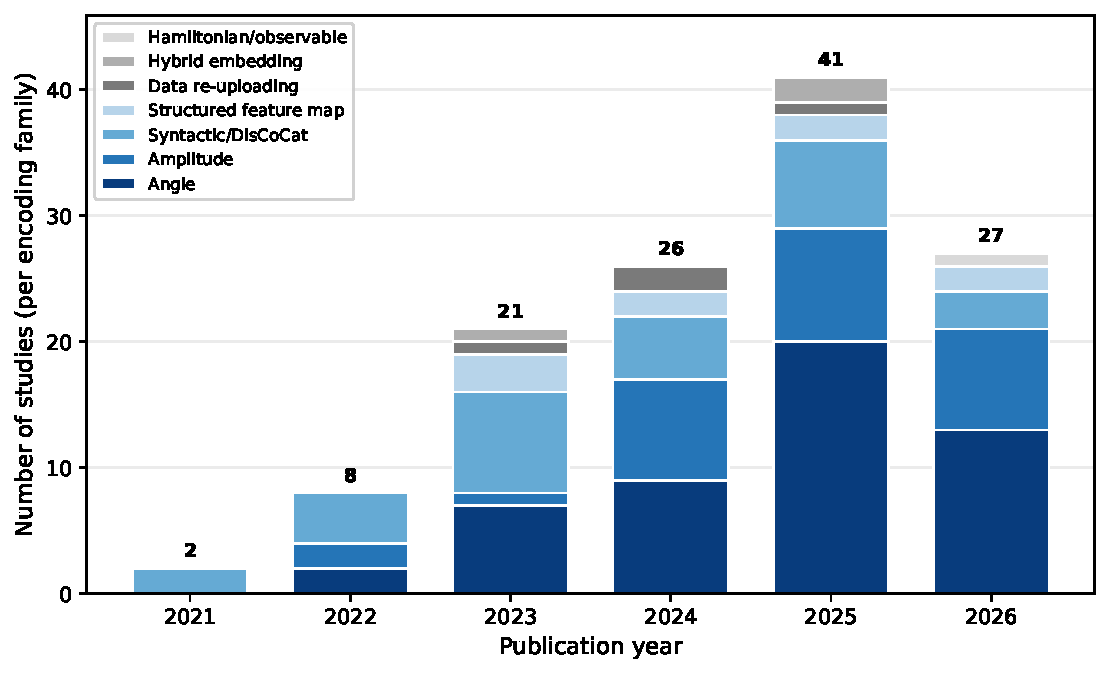
\includegraphics[width=\textwidth,height=0.42\textheight,keepaspectratio]{figures/encoding_by_year.pdf}
  \caption{Encoding family by publication year in the final corpus (2026 is a partial year at the time of the search).\label{fig:encoding_by_year}}
  \vspace{10mm}
  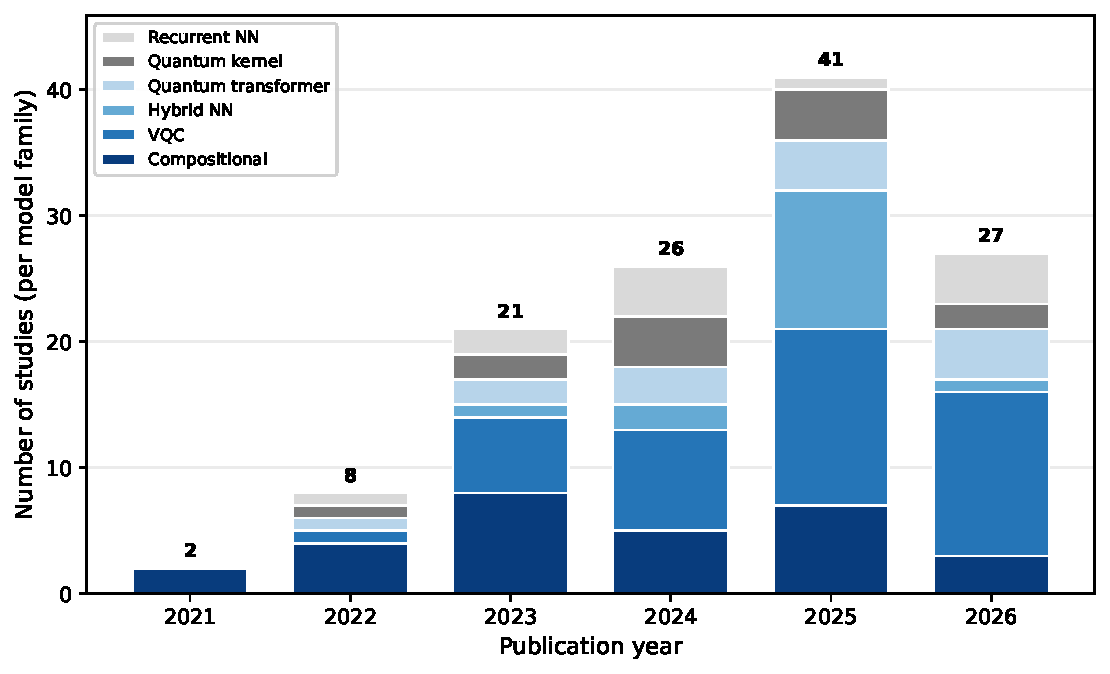
\includegraphics[width=\textwidth,height=0.42\textheight,keepaspectratio]{figures/model_family_by_year.pdf}
  \caption{Model family by publication year in the final corpus (2026 is a partial year at the time of the search).\label{fig:model_family_by_year}}
  \end{figure*}

The previous sections analyzed each encoding as a cross-section of the corpus, without regard to time. This section answers RQ3 by adding publication year, the dimension held constant so far, and describes how much the field has grown and how its composition changed as it grew. The final corpus spans six publication years, from two studies in 2021 to 8, 21, and 26 in the next three years and a peak of 41 in 2025. The last year, 2026, has 27 studies but was incomplete at the time of writing, because the search preceded the end of the year. Any apparent decline in 2026 is therefore an artifact of the search cutoff and is not treated as a contraction.

\subsection{Growth and the Changing Encoding Mix}
\label{subsec:temporal_encoding}

Figure~\ref{fig:encoding_by_year} breaks down the fivefold growth of the field since 2022 by encoding family. Four movements account for it.

\begin{itemize}
\item Syntactic/DisCoCat encoding loses share without shrinking. It is the only family present in 2021 and still holds half the corpus in 2022, then falls steadily to 38\% in 2023, 19\% in 2024, and 11\% in 2026, while its absolute count stays between two and eight studies a year. The decline is relative, because the field grew around a family that did not contract.

\item Angle encoding absorbs most of the new volume. Its share rises from a quarter of the yearly corpus in 2022 to roughly half from 2025, and its count from two studies to 20.

\item Amplitude encoding stabilizes together with transformer embeddings. After a quarter of the small 2022 corpus and a drop below 5\% in 2023, it holds between a fifth and a third of every year from 2024 on. From the same year, every VQC-hosted amplitude study runs on dense transformer embeddings (Section~\ref{subsec:amplitude_across_families}).

\item The other families stay marginal. Structured feature maps remain in single digits apart from 14\% in 2023, and the three emerging families together never exceed a tenth of the output of any year.
\end{itemize}

Taken together, the two vector-loading encodings rise from half of the 2022 corpus and 38\% of 2023 to 65\% in 2024, 71\% in 2025, and 78\% in the partial 2026 count. One possible explanation is a difference in barrier to entry. No paper in the corpus frames its encoding choice in these terms, so this remains a hypothesis suggested by the aggregate counts. A DisCoCat study commits to a grammar formalism, a parser that can produce pregroup or CCG derivations, and the narrow \textsc{lambeq}/\textsc{DisCoPy} toolchain, and it pays that cost again for every new sentence, language, or domain (Section~\ref{subsec:syntactic_across_ansatze}). Angle and amplitude encoding require only a fixed-length numeric vector. Once pretrained embeddings became a routine input, the marginal cost of a new study fell to that of an off-the-shelf VQC or kernel recipe already circulating in the broader quantum machine learning literature. The families that stayed marginal still require bespoke engineering, such as a decomposed recurrent layer, a co-designed classical encoder, or a custom observable construction. Their output therefore scales with the number of researchers willing to do that work, and not with the size of the field.

\subsection{From Compositional Monoculture to Architectural Pluralism}
\label{subsec:temporal_model_family}

Figure~\ref{fig:model_family_by_year} shows the same development from the architecture side. Compositional QNLP and syntactic encoding are the same 29 studies, so the compositional decline, from the entire 2021 corpus to half of 2022 and 11\% by 2026, is the same erosion seen on a second axis and not independent evidence. Three groups of architectures take over, 
%that share.
let summarize their trends below.  
\begin{itemize}
\item VQCs gain the most, from an eighth of the 2022 corpus to about a third by 2025 and just under half in 2026. A VQC is not specific to QNLP: Section~\ref{sec:comparative_analysis} showed it to be the default host for both angle and amplitude encoding, because it requires nothing of the input beyond a numeric vector. In 2025 and 2026, all but three of its 27 studies use one of the two.

\item Quantum transformers and kernels stay steady. Both hold between roughly 7\% and 15\% of each year from 2022 onward. Each requires a deliberately quantum-native design decision (a state-overlap readout or an attention-like circuit structure) that cannot be copied from a generic VQC recipe.

\item Hybrid neural models are the outlier. They are negligible through 2024, reach 27\% of the 2025 corpus, and fall back to 4\% in the partial 2026 count. Seven of the eleven hybrid studies of 2025 use angle encoding, so this jump and the rise of angle encoding in the same year are partly the same studies. This is also the architecture that gives the quantum component the smallest role, and the one that Section~\ref{subsec:emerging_specialized_interfaces} identified as hardest to attribute to that component.
\end{itemize}

Recurrent models, the remaining family, show no trend, with one to four studies a year since 2022. The 2026 column is partial throughout, so no fall recorded there can yet be read as a reversal. The two axes are consistent with each other: the fastest-growing segments are those with the lowest entry cost for a researcher who brings a pretrained classical model and a small amount of quantum machinery, and not those built around a bespoke quantum-native design. On this reading, the growth of the field has followed the path of least engineering effort, and not the encodings and architectures that Section~\ref{sec:taxonomy} judged most linguistically or computationally motivated.

\section{Task-Level Fit Between Encoding and Model Family}
\label{sec:task_fit}

Sections~\ref{sec:comparative_analysis} and~\ref{sec:temporal_evolution} established which encoding a study uses and when. This section answers RQ4: whether that choice ever follows the task, that is, whether any task family gives a principled reason to prefer one encoding, and whether the field acts on it. The analysis is structural. It considers what an encoding computes and not the reported results, because the corpus provides no basis for comparing the performance figures of two studies.

\Figure[t!](topskip=0pt, botskip=0pt, midskip=0pt)[width=\textwidth]{figures/encoding_by_task_family.pdf}{Encoding family by NLP task family in the final corpus. A study evaluating several task families is counted once in each.\label{fig:encoding_task}}

As Figure~\ref{fig:encoding_task} shows, sentiment and other text classification together account for most of the corpus and include every encoding family of any size.
These two task families say little about the fit between task and encoding, because the encoding mix within each reproduces the corpus-wide mix. Angle encoding takes 24 of the 51 sentiment studies and 21 of the 56 other-classification studies, amplitude 12 and 9, and syntactic 8 and 15, so no family's share within either task departs from its corpus-wide value by more than eight percentage points. The distribution is consistent with the corpus-wide habits documented in Sections~\ref{sec:comparative_analysis} and~\ref{sec:temporal_evolution}, mainly which toolchain and which pretrained embedding a group already had available, and not with any property of sentiment or topic classification.
Classification is thus the setting where the corpus has the most data and the least power to answer the question.

Similarity and disambiguation is the one task family in which a pattern with a mechanistic basis appears. Amplitude encoding accounts for six of the thirteen studies, roughly double its share of the corpus overall, although with thirteen studies this enrichment is only suggestive.
The argument rests on the mechanism more than on the count, and Section~\ref{subsec:amplitude_across_families} already established it. The inner product of two amplitude-encoded states is a cosine similarity, so a SWAP test or overlap measurement performs the core computation of the task and does not merely feed a downstream classifier. The same mechanism explains why three of those six studies are quantum-kernel models \cite{cavar_word_2025,cavar_old_2026,cavar_semantic_2024}: a kernel method is little more than a trained readout around that overlap.
What the fit delivers is feasibility and not superiority, as those three studies state themselves. Their contribution is that the encoded state reproduces classical embedding similarity with minimal loss at logarithmic qubit cost. An amplitude state loads the classical geometry it is given, so an overlap readout can reproduce a classical cosine similarity faithfully but has no means of improving on it. The fit also follows from the definition of amplitude encoding and was not found by systematic search: no study in the corpus set out to compare encodings on similarity tasks.

Relational tasks (question answering and, to a lesser extent, similarity itself) show a weaker version of the same logic on the compositional side, but here the corpus is too thin to test anything.
Syntactic/DisCoCat encoding takes two of the seven question-answering and retrieval studies and five of the thirteen similarity and disambiguation studies. This is consistent with the intuition that grammatical structure should matter most when a task is explicitly about how words or entities relate. With such denominators, however, the departure from the corpus-wide share proves nothing, since one study more or less moves the question-answering share by fourteen percentage points.
The structural argument also conflicts with the practical constraint documented in Section~\ref{subsec:syntactic_across_ansatze}. The family becomes less practical as a task departs from short, curated sentences, and relational tasks are both where compositional structure is best motivated and where the grammar-to-circuit pipeline is under the most strain. The few studies available cannot settle which of the two effects dominates.

Sequence labeling, question answering, and generation or language modeling are each covered by only six to ten studies, too few to support a claim either way, but for different reasons. Sequence labeling is almost entirely angle-encoded (five of its six studies), so there are no alternatives to compare within the cell. Question answering and generation are spread thinly across several encodings, but each pairing consists of one or two papers from a single research thread, and no second, independent group has reproduced it.

Three studies fall outside the six task families. Two are quantum topic models \cite{kabir_qtopic_2026,qiao_quantum_2024}. Both are unsupervised and evaluated by topic coherence and diversity, not against labels, so they fit neither the supervised families nor generation. One uses angle encoding and the other amplitude, which settles nothing. The third is Quanthoven \cite{miranda_quantum_2022}, which trains DisCoCat circuits to classify and then compose music. It is the one study in the corpus whose task is not linguistic, and it is retained because its grammar-to-circuit pipeline is the same construction the compositional family uses on text.

The central finding of this section is therefore methodological and not about performance, and it is what justifies the structural reading used throughout. The corpus cannot be pooled on results, because each study selects its own dataset, its own classical comparison, and its own evaluation protocol. The 125 studies name 141 distinct datasets, and 122 of them are used by exactly one paper (Section~\ref{subsec:reproducibility_gap}). The classical systems used for comparison are nearly unique to each paper as well, and 15 studies report no classical baseline at all. A reported accuracy figure in this corpus is thus a statement about one pipeline, on one dataset, against one baseline. The difference between two such figures from two different studies cannot be attributed to the encoding that distinguishes them. For this reason the one fit between task and encoding that the corpus does support has to be argued from mechanism, since it cannot be measured from results, and even that fit concerns efficiency and not superiority.

\section{Experimental Rigor: Simulation, Hardware, and Reproducibility}
\label{sec:experimental_rigor}

This section answers RQ5 by assessing how rigorously the corpus tests the choices described so far. Every study was coded for its execution regime, simulation framework, code availability, and whether scalability was discussed. The question is how much evidence supports the claim that an encoding works.

\subsection{Execution Regimes Across the Corpus}
\label{subsec:execution_regimes}

Noiseless statevector simulation dominates: 96 out of 125 studies (76.8\%) report exact simulation only. A further 16 (12.8\%) simulate under an explicit noise model, and 11 (8.8\%) pair simulation with a hardware validation run. Only two studies (1.6\%) run exclusively on real hardware, a quantum-kernel KNN classifier \cite{zeguendry_quantum_2024} and a quantum self-attention model on a 72-qubit superconducting processor \cite{he_training_2024}. The mixed and hardware-only studies together give 13 hardware-touched studies (10.4\%), and adding noisy simulation gives 29 studies (23.2\%) with any noise or hardware engagement. A study counts as hardware-touched only if it names the device.

Table~\ref{tab:execution_by_encoding} reports execution regime for each encoding family exploiting the taxonomy of Section~\ref{sec:taxonomy}. Four of the seven families have fewer than ten studies, so most per-family percentages are descriptive only. Syntactic/DisCoCat encoding engages noise or hardware at about twice the rate of angle and amplitude encoding (34.5\% against 16.5\%), because its \textsc{lambeq}/\textsc{DisCoPy}/\textsc{pytket} stack has direct IBM Quantum integration and its shallow circuits are cheap to queue on real devices \cite{lorenz_qnlp_2023,meichanetzidis_grammar-aware_2023,peral-garcia_comparing_2024,miranda_quantum_2022}. The one contrast with large enough denominators is that angle and amplitude encoding, 79 out of 125 studies, engage noise or hardware at less than half the rate of the rest of the corpus (13 out of 79, 16.5\%, against 16 out of 46, 34.8\%), and the same holds for real-device runs (5 out of 79 against 8 out of 46). These two encodings carry the growth of the field (Section~\ref{subsec:temporal_encoding}), so most of their reported accuracy figures (66 out of 79) come from noiseless simulation and say nothing about decoherence, gate error, or readout noise.

Hybrid embedding and Hamiltonian/observable encoding have no hardware or noisy-simulation validation at all. For Hamiltonian encoding this means that its central promise, avoiding the state-preparation cost of amplitude encoding, has not been tested under conditions that would stress it.

\subsection{Execution by Model Family and the Recurrent-Network Blind Spot}
\label{subsec:execution_by_model_family}

The same asymmetry appears across model families. Quantum kernels are the most hardware-touched (3 out of 13 on a named device, 23.1\%), consistent with their concentration in amplitude and structured-feature-map encoding. On the wider measure compositional models lead, with 34.5\% against 30.8\% for kernels, while VQCs, hybrid neural models, and quantum transformers lie between 19\% and 27\%. Recurrent quantum models do not have it at all, in fact, all the 12 studies report noiseless simulation only. A recurrent cell re-applies its encoding and ansatz once per token, so circuit depth and exposure to noise grow with sequence length. The family that relies the most on reusing a small register is thus the one for which noise robustness has been tested the least.


\begin{table}[t]
\caption{Execution regime by encoding family in the final corpus.}
\label{tab:execution_by_encoding}
\centering
\footnotesize
\renewcommand{\arraystretch}{1.15}
\setlength{\tabcolsep}{5pt}
\begin{tabular}{@{}lcccc@{}}
\noalign{\hrule height 0.8pt}
\textbf{Encoding family} & \textbf{Noiseless} & \textbf{Noisy sim.} & \textbf{Mixed} & \textbf{HW only}\\
\hline
Angle & 42 & 6 & 2 & 1\\
Amplitude & 24 & 2 & 1 & 1\\
Syntactic/DisCoCat & 19 & 6 & 4 & 0\\
Structured feature map & 5 & 1 & 3 & 0\\
Data re-uploading & 2 & 1 & 1 & 0\\
Hybrid embedding & 3 & 0 & 0 & 0\\
Hamiltonian/observable & 1 & 0 & 0 & 0\\
\noalign{\hrule height 0.8pt}
\end{tabular}
\end{table}

%\subsection{Hardware Validation Peaked in 2024 and Then Collapsed}
\subsection{Trends on Hardware Validation}
\label{subsec:hardware_timeline}

The corpus grew roughly twentyfold between 2021 and 2025, but the hardware-touched share did not grow with it: 0\% in 2021, 12.5\% in 2022, 14.3\% in 2023, 26.9\% in 2024, then 2.4\% in 2025 and 3.7\% in 2026 so far.
Pooled, 11 out of 57 studies published between 2021 and 2024 are hardware-touched (19.3\%), against 2 out of 68 in 2025 and 2026 (2.9\%). The two years with the highest output therefore have the lowest combined rates, 17.1\% and 18.5\% against 25\% to 35\% from 2022 to 2024. This matches the low-barrier explanation proposed in Section~\ref{subsec:temporal_encoding}: growth came through the protocol that asks least of a newcomer, a local noiseless simulator. The two recent studies that reach hardware are a neural-quantum-embedding pipeline on an IBM backend \cite{baik_neural_2025} and a quantum-secure federated-learning system on a 156-qubit backend \cite{liu_experimentally_2026}.

\subsection{Framework Fragmentation and the Reproducibility Gap}
\label{subsec:reproducibility_gap}

The tooling is not standardized even in simulation: the largest single category, 37 out of 125 studies (29.6\%), does not name its simulation framework. About the rest of the studies, \textit{PennyLane} is the most common one (43 studies, 21 of them using it exclusively), Qiskit is the second one (25 mentions, 9 exclusively), and \textsc{lambeq} anchors the syntactic subcorpus. The others mostly appear in a single papers, and outside this core the stacks built on top of the frameworks are close to unique per paper. Only 25 studies (20.0\%) report publicly available code. In all, 34 studies (27.2\%) report neither code nor framework and only 22 (17.6\%) report both, so a substantial part of the corpus cannot be re-run independently even in simulation.

Scalability is discussed by 91 studies (72.8\%), but each against a standard defined by the authors, from a formal resource analysis to a single sentence about future work. Together with the dominance of noiseless simulation, this leaves open whether any encoding of Section~\ref{sec:taxonomy} would still work outside a simulator at larger register sizes, which extends the state-preparation caution raised for amplitude encoding in Section~\ref{subsec:amplitude_encoding}.

\begin{table*}[t]
\caption{Open challenges, the corpus evidence behind each, and the proposed action.}
\label{tab:challenges}
\centering
\footnotesize
\renewcommand{\arraystretch}{1.15}
\setlength{\tabcolsep}{5pt}
\begin{tabular}{@{}l p{0.42\textwidth} p{0.33\textwidth}@{}}
\noalign{\hrule height 0.8pt}
\textbf{Challenge} & \textbf{Evidence in the corpus} & \textbf{Proposed action} \\
\hline
C1 Encoding bottleneck & \raggedright Embeddings of 768 dimensions cut to 10, 4, or 2 features; state-preparation cost left out of reported qubit budgets & \raggedright Report retained dimensionality and preparation depth; classical baseline on the reduced input \tabularnewline[2pt]
C2 Incommensurable evaluation & \raggedright Dataset, baseline, and protocol chosen study by study; 15 studies without a classical baseline & \raggedright Shared benchmarks with fixed classical baselines; controlled comparisons \tabularnewline[2pt]
C3 Simulation-to-hardware gap & \raggedright 96 of 125 studies noiseless only; hardware-touched share from 26.9\% in 2024 to 2.4\% in 2025 & \raggedright Calibrated noise model as the minimum for publication \tabularnewline[2pt]
C4 Absent scaling evidence & \raggedright 102 of 125 studies evaluate a single register width & \raggedright Register-width sweeps \tabularnewline[2pt]
C5 Reproducibility & \raggedright 100 studies release no code; 37 name no framework; 122 of 141 datasets used by one paper & \raggedright Released code, named framework, shared benchmarks in place of toy corpora \tabularnewline
\noalign{\hrule height 0.8pt}
\end{tabular}
\end{table*}

\section{Trends and Open Challenges}
\label{sec:trends_challenges}

Read together, the previous sections describe a field whose growth and whose evidence are moving apart. The growth is a consolidation on angle and amplitude encoding, the two encodings that ask least of a newcomer. The same two encodings are the least validated: 2025 and 2026, the years of fastest growth, have the lowest combined rate of hardware or noisy-simulation engagement since 2022, and the shortfall concentrates in these families. The one fit between task and encoding that has a mechanistic basis, amplitude encoding on similarity and disambiguation, remains a small niche. Because results cannot be compared across studies, a reported figure says little beyond the pipeline that produced it. These gaps do not belong to one encoding or one model family. They come from how the field runs and reports its experiments, and they translate into the five challenges of Table~\ref{tab:challenges}, each discussed below together with the action it calls for.

\subsection{Open Challenges and an Agenda for Future Work}
\label{subsec:open_challenges}
\label{subsec:future_agenda}

\begin{enumerate}
\item[C1)] \textbf{The encoding bottleneck.} Every non-syntactic encoding has to bridge the gap between the dimensionality of a useful text representation and the qubit budget of near-term hardware, and each pays for it in lost information, circuit depth, or classical preprocessing. In the corpus, embeddings of 768 dimensions are reduced to ten, four, or two features before the circuit \cite{ahmad_hybrid_2023,kumar_hybrid_2026,altintas_beyond_2025}, and state-preparation cost is routinely left out of the reported qubit budget. The proposed mitigations \cite{zhang_entangled_2024,tiblias_efficient_2026,silver_lexiql_2024} change which cost is paid, and no study measures what the reduction removes. Studies should report the retained dimensionality and the preparation depth alongside the qubit count, and the result of a classical model on the same reduced input.

\item[C2)] \textbf{Incommensurable evaluation.} Dataset, classical comparison, and protocol are chosen study by study, and 15 studies report no classical baseline. Even the one structurally motivated pairing, amplitude encoding on similarity tasks, is presented by its own study as a reproduction of classical similarity rather than an improvement over it \cite{cavar_word_2025,cavar_old_2026}. A small set of shared, encoding-agnostic benchmarks with fixed classical baselines would let a future meta-analysis attribute a performance gap to the encoding and not to the baseline a group selected. Controlled comparisons that hold model family, dataset, and circuit depth fixed and vary only the encoding or ansatz would separate the encoding from the architecture it is usually bound to.

\item[C3)] \textbf{The gap between simulation and hardware.} Real-device validation peaked in 2024 and then fell sharply; the only hardware-validated studies of 2025 and 2026 are just two studies \cite{baik_neural_2025,liu_experimentally_2026}. Noiseless simulation says nothing about decoherence, gate error, or readout noise, the properties that decide near-term viability. Accuracy under an explicit, calibrated noise model should therefore be the minimum for publication, especially for angle and amplitude encoding and for recurrent architectures, which have no noisy-simulation or hardware study in the corpus.

\item[C4)] \textbf{Absent scaling evidence.} Only 23 studies reports test with more than one register width, and systematic sweeps such as the comparisons from 1 to 16 qubits in \cite{zhang_entangled_2024,kim_quantum_2025} are rare. The resource arguments made for each encoding are asymptotic, while the evidence is a single point. A register-width sweep should accompany any claim about scaling.

\item[C5)] \textbf{Reproducibility and trivial benchmarks.} Most studies release no code, and many do not name their simulation framework. Only 7 datasets recur in four or more papers: generic sentiment benchmarks with no QNLP-specific signal (IMDb, 12 papers; Amazon reviews, 8; Yelp, 7) and the synthetic MC and RP corpora of about 100 sentences built into \textsc{lambeq} (12 and 9 papers), on which near-perfect accuracies are reported \cite{lorenz_qnlp_2023,bouakba_ensemble_2023,liu_research_2024}. Releasing code, naming the framework and backend, and replacing toy corpora with the shared benchmarks of C2 would make independent re-execution possible.
\end{enumerate}

One further direction goes beyond repairing current practice. The single documented fit between task and encoding yields efficiency and not a better result, because the encoded state reproduces the classical geometry it loads. Future work should look deliberately for tasks in which the mathematical structure of an encoding performs the core computation and that computation is classically expensive. Relational tasks such as question answering, where syntactic encoding has a theoretical fit that the corpus is too thin to evaluate, are one candidate. A targeted study of this kind, as opposed to another general-purpose classifier, could show whether a structural fit ever produces a gain against a fixed classical baseline.

\section{Conclusion}
\label{sec:conclusion}

This survey isolated text encoding as the unit of analysis in QNLP and classified 125 studies published between 2021 and 2026 into seven encoding families. Its central result is that the literature cannot yet answer the question it implicitly poses, which encoding works better for language. What the corpus does support is structural: every non-syntactic family resolves the encoding bottleneck by choosing which cost to pay, discarded information, circuit depth, or classical preprocessing.

The corpus also shows what is missing. No study holds model family, dataset, and circuit depth fixed while varying only the encoding, and few report the retained dimensionality, the state-preparation cost, or a classical baseline on the same reduced input. These are the measurements that would turn the structural reading of this survey into an empirical one, and the agenda of Section~\ref{sec:trends_challenges} is built around them.

Until such studies exist, encoding should be reported and justified as a design choice in its own right, with the same care given to the ansatz, the optimizer, and the classical baseline.

\bibliography{references}
\bibliographystyle{IEEEtran}

\EOD

\end{document}
